% LaTeX template for Avantprojecte (TFG Initial Proposal)
% 
% Author: Eloi Egea Rada
% © 2025, Eloi Egea Rada
% Licensed under CC BY-NC-SA 4.0
% Template for Final Degree Projects at Centre Universitari TecnoCampus

\documentclass[a4paper, twoside, 12pt, openany]{report}

% ============================================================================
% PREAMBLE — Packages and configuration
% ============================================================================

% --- Typography with XeLaTeX/LuaLaTeX ---
\usepackage{fontspec}
\usepackage{verbatim}
\usepackage{graphicx}
\usepackage{float}
\usepackage[english]{babel}
\usepackage{csquotes}
\usepackage{eurosym}

\usepackage{fancyhdr} % Header and footer customization
\usepackage{etoolbox} % Page numbering style control
\usepackage{geometry} % Margin configuration
\usepackage{setspace} % Line spacing adjustment
\usepackage{titlesec} % Section and chapter title formatting
\usepackage[nottoc, numbib]{tocbibind} % Auto-include bibliography and indexes in ToC
\usepackage[nonumberlist, toc]{glossaries} % Glossary generation
\usepackage[style=ieee, backend=biber]{biblatex} % Bibliography management in IEEE format

% Complex tables for time tracking
\usepackage{array}
\usepackage{tabularx}
\usepackage{booktabs}
\usepackage{longtable}
\usepackage{listings}
\lstset{
    basicstyle=\ttfamily\small,
    breaklines=true,
    breakatwhitespace=true,
    frame=single,
    numbers=left,
    numberstyle=\tiny,
    numbersep=5pt,
    showstringspaces=false,
    captionpos=b
}
% Hyperlinks (load AFTER other packages)
\usepackage{amssymb}
\usepackage{hyperref}

% ============================================================================
% OPENDYSLEXIC FONTS SELECTION
% ============================================================================

\setmainfont{OpenDyslexic}[
    Path = /usr/share/fonts/opentype/opendyslexic/,
    Extension = .otf,
    UprightFont = *-Regular,
    BoldFont = *-Bold,
    ItalicFont = *-Italic,
    BoldItalicFont = *-BoldItalic
]

\setsansfont{OpenDyslexicAlta}[
    Path = /usr/share/fonts/opentype/opendyslexic/,
    Extension = .otf,
    UprightFont = *-Regular,
    BoldFont = *-Bold,
    ItalicFont = *-Italic,
    BoldItalicFont = *-BoldItalic
]

\setmonofont{OpenDyslexicMono}[
    Path = /usr/share/fonts/opentype/opendyslexic/,
    Extension = .otf,
    UprightFont = *-Regular
]

% ============================================================================
% LOAD GLOSSARY
% ============================================================================



% Load glossary definitions from an external file
\input{../../resources/glossary.tex}
\setglossarystyle{altlist}
\setacronymstyle{long-short}
\makeglossaries
\addbibresource{../../resources/references.bib} % El fitxer .bib amb les referències


% ============================================================================
% TITLE FORMATTING
% ============================================================================

\titleformat{\chapter}[block]{\normalfont\fontsize{18pt}{0pt}\bfseries}{\thechapter}{1em}{}
\titlespacing*{\chapter}{0pt}{0pt}{\baselineskip}

\titleformat{\section}[block]{\normalfont\fontsize{16pt}{0pt}\bfseries}{\thesection}{1em}{}
\titleformat{\subsection}[block]{\normalfont\fontsize{14pt}{0pt}\bfseries}{\thesubsection}{1em}{}

% ============================================================================
% HYPERLINK CONFIGURATION
% ============================================================================

\hypersetup{
    colorlinks=true,
    linkcolor=black,
    citecolor=black,
    filecolor=magenta,
    urlcolor=blue,
    pdftitle={Ethical Pentesting in Virtualized Environments with EVE-NG},
    pdfauthor={Eloi Egea Rada},
    pdfpagemode=FullScreen
}

% ============================================================================
% PAGE MARGINS CONFIGURATION
% ============================================================================

\geometry{top=3cm, bottom=2.54cm, left=2.54cm, right=2.54cm, bindingoffset=0.46cm}
\setlength{\headheight}{14.5pt}


\setlength{\parindent}{0pt} % Disable paragraph indentation


% Imatges
\graphicspath{{../../images/}}


% ============================================================================
% COVER PAGE & PRELIMINARIES
% ============================================================================

\fancypagestyle{plain}{
    \fancyhf{}
    \fancyhead[RO,LE]{\fontsize{10}{12}\textit{\thepage}}
    \fancyhead[RE]{\fontsize{10}{12}\textit{Ethical Pentesting in Virtualized Environments with EVE-NG}}
    \fancyfoot{}
}

\pagestyle{plain}

\title{
        \begin{figure}
            \centering
            
\includegraphics[width=0.85\linewidth]{../../images/logo-tecnocampus.png}
        \end{figure}
        
        \fontsize{14pt}{0pt}\textbf{Bachelor in Computer Engineering — Management and Information Systems} \\
        
        \vspace*{2cm}

        \textbf{Ethical Pentesting in Virtualized Environments with EVE-NG} \\

        \vspace*{1cm}

        \textbf{Memory} \\
        \textbf{Volume I}

        \vspace*{5cm}
}

\author{
\fontsize{14pt}{0pt}
	\textbf{Eloi Egea Rada} \\
	\textbf{Supervisor: Pere Vidiella i Catalan}
}

\date{April 2026}

\begin{document}

% === COVER PAGE ===
\maketitle

\newpage
\thispagestyle{empty}
\null
\newpage

% ============================================================================
% TABLE OF CONTENTS & PRELIMINARY PAGES
% ============================================================================

\pagenumbering{Roman}

\tableofcontents
\listoffigures
\listoftables



\onehalfspacing
\setlength{\parskip}{12pt}
\glsaddall
\printglossaries


\newpage

\fancypagestyle{plain}{
    \fancyhf{}
    \fancyhead[RO,LE]{\fontsize{10}{12}\textit{\thepage}}
    \fancyhead[LO]{\fontsize{10}{12}\textit{\nouppercase{\textit{\leftmark}}}}
    \fancyhead[RE]{\fontsize{10}{12}\textit{Ethical Pentesting in Virtualized Environments with EVE-NG}}
    \fancyfoot{}
}

\pagestyle{plain}

\pagenumbering{arabic}

% ============================================================================
% DEDICATION
% ============================================================================
% ============================================================
% Dedication page -- no heading, Juanola style
% ============================================================
\thispagestyle{empty}
\null\vfill
\begin{flushright}
\begin{minipage}{0.62\textwidth}
\textit{I dedicate this thesis to my grandmother,\\
who passed away just before I began my degree---
shortly after my university admission
and the day before my English examination.
Choosing to write this thesis in English is,
in part, a way to close a chapter
that marked the beginning of my university journey
without the person who meant most to me,
and who, in many ways, was like a mother to me.}
\end{minipage}
\end{flushright}
\vfill\null\newpage

% ============================================================
% Acknowledgements -- same visual style, small simulated title
% ============================================================
\thispagestyle{empty}
\null\vfill
\begin{flushright}
\begin{minipage}{0.62\textwidth}
{\normalfont\large\bfseries Acknowledgements}\\[0.8em]
{\itshape
I would like to express my sincere gratitude to my tutor,
Pere Vidiella~i~Catalan, for his guidance, availability,
and constructive feedback throughout this project.
His trust and technical insight have been decisive in shaping
both the scope and the academic rigour of this work.

\medskip
I am also deeply grateful to my friends, my partner, and my partner's
family for their unwavering support throughout my studies---especially
during a period when I faced a serious health challenge.
Their presence, care, and belief in me have been essential to
reaching this point.

}
\end{minipage}
\end{flushright}
\vfill\null\cleardoublepage


% ============================================================================
% CHAPTER 1: INTRODUCTION
% ============================================================================


% Document: TFG Avantprojecte - Object of the Project
% Language: English

\chapter{Introduction}

%\section{Problem Statement and Educational Gap}

Cybersecurity education faces a critical challenge: the disconnect between
theoretical knowledge of IT systems and practical understanding of how
security failures manifest in integrated environments. While students in
the Computer Engineering degree program learn fundamental concepts in databases,
network protocols, operating system internals, and software architecture,
they rarely experience how misconfigurations and design flaws in these domains
directly translate to security vulnerabilities.

Current training approaches amplify this gap. Commercial platforms such as
HackTheBox\cite{hackthebox} and TryHackMe\cite{tryhackme} focus on isolated challenge-based scenarios that
abstract away system complexity. Professional pentesting certifications
(e.g., CEH, OSCP\cite{ceh_framework,oscp_exam}) expect hands-on experience in realistic environments, yet
many academic programmes struggle to provide such environments due to cost,
complexity, or vendor lock-in.

Within the TecnoCampus Bachelor's Degree in Computer Engineering
(Management and Information Systems track), the ``Introduction to Cybersecurity''
course currently lacks a structured, reusable, and automatable lab environment that:

\begin{itemize}
    \item Aligns pentesting scenarios with specific degree learning outcomes
    \item Enables students to recognise vulnerabilities within integrated systems
          (not isolated exploits)
    \item Provides reproducible environments for consistent assessment
    \item Reduces instructor workload through automation and documentation
    \item Remains cost-effective and institution-independent (open-source,
          locally maintained)
\end{itemize}

\section{Context}

The Centre Universitari TecnoCampus~\cite{tecnocampus} offers applied science degrees
oriented towards professional practice in technology, business, creative industries,
and health. Affiliated with the Universitat Pompeu Fabra, it carries that
university's quality seal. Established in 2023 through the merger of three schools---the
Escola Superior Politecnica (ESUPT), the Escola Superior de Ciencies Socials i de
l'Empresa (ESCSET), and the Escola Superior de Ciencies de la Salut (ESCST)---it is
located at the technology park of the same name in Mataro, combining academic
infrastructure with an entrepreneurial ecosystem that facilitates student participation
in innovation and industry-facing projects.

The primary beneficiary of this project is the Bachelor's Degree in Computer
Engineering (Management and Information Systems track). Students in this programme
acquire foundational competencies in networks, operating systems, databases, and
software engineering all of which are directly relevant to security practice.
The \textit{Introduction to Cybersecurity} course is a natural integration point
for these skills, yet it currently lacks a dedicated hands-on environment.

Three perspectives illustrate the gap this project addresses:

\paragraph{Institutional perspective.}
The absence of dedicated cybersecurity lab infrastructure limits the institution's
capacity to offer competitive, hands-on security training aligned with degree
learning outcomes. Commercial alternatives such as HackTheBox and TryHackMe are
externally hosted, non-customisable, and not designed to map to specific academic
curricula or assessment rubrics.

\paragraph{Student perspective.}
Students encounter security concepts as isolated theoretical constructs rather than
as failures observable in realistic, integrated environments. Without exposure to
multi-component systems---firewalls, routers, servers, and applications working
together---they cannot develop the diagnostic reasoning required in professional
security roles.

\paragraph{Instructor perspective.}
Designing and maintaining practical security exercises is resource-intensive.
The absence of reusable, automatable lab environments forces instructors to
improvise or rely on third-party platforms, reducing pedagogical control and
limiting reproducibility across cohorts.

\section{Proposed Solution}

This project proposes a reusable penetration testing lab package built on
EVE-NG~\cite{eve_ng} and deployed on self-hosted infrastructure, designed
specifically for the \textit{Introduction to Cybersecurity} course at TecnoCampus.
The package comprises four progressive lab scenarios covering network reconnaissance
and enumeration, web application vulnerabilities, incident response and log forensics, and
privilege escalation. Labs~1--3 are fully implemented and validated; Lab~4
(privilege escalation) is in progress and will be completed in Phase~3. Each lab is self-contained: it includes an EVE-NG topology
file (\texttt{.unl}), a student guide (\textit{enunciado}) and an instructor
resolution guide (\textit{resolució}), an assessment rubric, and supporting
configuration and automation scripts. The entire package is open-source, vendor-
independent, and deployable on any institution running a compatible hypervisor.
Instructor deployment references, credentials, and lab-specific configuration
details are compiled in the Annexos (Volume~II), which accompanies this memory
and is also published online at \path{docs/web/docs/assets/official\_Documents/annexos.md}.



% ============================================================================
% CHAPTER 2: STATE OF THE ART
% ============================================================================


% ============================================================
% Autor: Eloi Egea Rada
% Tema: Existing solutions, platforms, and gap analysis
% ============================================================

\chapter{State of the Art}
\label{ch:state-of-art}

Cybersecurity education has experienced exponential growth over the past decade, driven by
increasing industry demand for skilled professionals and the accessibility of online learning
platforms. While students have unprecedented access to training resources, the fragmentation
of educational approaches has created gaps between abstract theoretical knowledge and practical,
integrated system security. This chapter examines existing platforms and methodologies, identifies
gaps in current offerings, and positions this bachelor's thesis within the broader context of
cybersecurity pedagogical innovation.


\section{Existing Platforms Overview}

The major platforms used for cybersecurity training share a common limitation: they are designed
for independent learners or certification preparation rather than curriculum-aligned institutional
deployment. Table~\ref{tab:platform_comparison} summarises their key characteristics.
Platforms such as HackTheBox~\cite{hackthebox} and TryHackMe~\cite{tryhackme} are externally hosted
and cannot be deployed on institutional infrastructure. SEED Labs~\cite{seedlabs} and
GOAD~\cite{goad} support local deployment but cover only isolated concepts or narrow domains.
VulnHub~\cite{vulnhub} and Hack4u~\cite{hack4u} lack automation and assessment integration.
Cisco Networking Academy~\cite{cisco_netacad} provides formal structure but is tightly coupled
to vendor technology and limited to network simulation.

\begin{table}[H]
\centering
\scriptsize
\setlength{\tabcolsep}{4pt}
\begin{tabularx}{\textwidth}{lXXXXX}
\toprule
\textbf{Platform} & \textbf{Approach} & \textbf{Deploy} & \textbf{Curriculum} & \textbf{Auto} & \textbf{Network} \\
\midrule
HackTheBox & CTF & No & Minimal & No & Isolated \\
TryHackMe & Gamified & No & Structured & No & Limited \\
Cisco Academy & Academic & Yes (PT) & Strong & Limited & Net-focused \\
SEED Labs & Conceptual & Yes (Docker) & Concept-based & Minimal & Isolated \\
GOAD & AD-focused & Yes (\mbox{Terraform}) & None & Moderate & \mbox{AD Domain} \\
VulnHub & Community & Yes & None & No & Isolated \\
Hack4u Academy & Methodology & External & Strong & Minimal & Limited \\
\bottomrule
\end{tabularx}
\caption{Comparative Analysis: Existing Cybersecurity Training Platforms}
\label{tab:platform_comparison}
\end{table}

Full individual platform descriptions, including detailed discussion of each platform's
pedagogical approach, deployment model, and specific limitations, are provided in
Appendix~\ref{app:platforms}.

\section{Security Frameworks and Methodologies}

Several authoritative frameworks inform cybersecurity education and guide both attack
methodologies and defensive best practices.

\subsection{OWASP Top 10}

The OWASP Top 10 is a regularly updated list of the most critical web application security
vulnerabilities \cite{owasp2021}. For educational purposes it provides a focused, industry-recognised
curriculum that prioritises the attack vectors students are most likely to encounter in practice.
Lab 2 of this project is directly aligned with OWASP Top 10 categories.

\subsection{CIS Critical Controls}

The CIS Critical Controls (v8.0) represent a prioritised set of defensive techniques spanning
network defence, data protection, and incident response \cite{cis_controls}. Labs 1 and 3
incorporate defensive controls so that students understand not only how to attack but why
specific security measures are implemented.

\subsection{NIST Cybersecurity Framework}

The NIST Cybersecurity Framework organises security activities into five functions: Identify,
Protect, Detect, Respond, and Recover \cite{nist_framework}. The lab design follows these
principles by enabling students to identify vulnerabilities through hands-on exercises and
understand corresponding protective measures.




\section{Prior Academic Research}

Academic research consistently validates the effectiveness of hands-on, laboratory-based
approaches in cybersecurity education. Conti and Di Pietro \cite{conti2019} demonstrate that
challenge-based environments significantly improve skill retention and practical competency
compared to purely theoretical instruction. Murphy et al.\ \cite{murphy2018} provide a
structured methodology for designing laboratory exercises that are explicitly aligned with
curriculum outcomes, validating the need for scenario-specific tasks and integrated
assessment. Sponj and Heri\v{c}ko \cite{sponj2021} conducted a systematic review of
cybersecurity education research, identifying hands-on practice and authentic task design as
the two most influential factors in learner engagement and competency development.
Al~Mohanadi and Furnell \cite{almohannadi2016} further establish a requirements-driven
approach to information security assessment laboratories, emphasising that lab tasks must
map directly to defined learning outcomes to achieve meaningful pedagogical impact.

These findings directly inform the design choices in this project: each lab is built around
scenario-based flags mapped to specific learning objectives, includes an instructor reference
sheet, and culminates in an automated assessment mechanism, addressing the gap between
platform availability and curriculum integration identified in the prior literature.

\section{Gap Analysis: What Existing Solutions Miss}

Despite the proliferation of cybersecurity training platforms, significant gaps remain:

\textbf{Gap 1: Curriculum Integration.}
Most platforms target independent learners or certification preparation rather than integration
into specific degree programmes. No major platform explicitly maps pentesting scenarios to the
learning outcomes of a particular computer science curriculum.

\textbf{Gap 2: Institution Control.}
Effective educational deployment requires institutional control over content, assessment, and
infrastructure. External platforms introduce dependencies and limit customisation, while
fully self-hosted solutions often impose high maintenance burdens.

\textbf{Gap 3: Integrated Network Penetration Testing.}
Most platforms focus on isolated services or individual techniques. Few provide realistic,
multi-system network topologies where reconnaissance informs a complete attack chain and
lateral movement is required.

\textbf{Gap 4: Automation and Scalability.}
Even classroom-oriented platforms often lack automated deployment, environment reset, and
assessment mechanisms, increasing instructor workload and limiting large-scale institutional
adoption.

\textbf{Gap 5: Balance of Guidance and Autonomy.}
Effective labs must balance sufficient structure to keep students on target with sufficient
openness to encourage problem-solving and methodology development.


\section{The Need for EVE-NG Based Labs}

This analysis reveals that while excellent individual components exist---gamified learning
(TryHackMe), challenging scenarios (HackTheBox), research-backed content (SEED Labs),
specialised domains (GOAD)---no existing solution comprehensively addresses the needs of a
university cybersecurity education programme:

\begin{itemize}
    \item \textbf{Curriculum-aligned labs}: Mapped to specific degree learning outcomes
    \item \textbf{Integrated network scenarios}: Multi-system penetration testing with realistic complexity
    \item \textbf{Institutional control}: Locally deployable, customisable, and maintainable
    \item \textbf{Complete automation}: One-command deployment and reset with built-in assessment
    \item \textbf{System-level realism}: Full virtual machine workflows (real OS images, ISO-based
          installation, native kernel behaviour) that reproduce the technical conditions of
          professional pentesting practice
\end{itemize}

The bachelor's thesis project bridges this gap by leveraging EVE-NG \cite{eve_ng} to create a
comprehensive, reusable, and automatable teaching package for cybersecurity practical labs,
synthesising the pedagogical strengths of existing platforms while addressing their limitations
through institutional control, curriculum alignment, and automation.


% END OF CHAPTER 2: STATE OF THE ART



% ============================================================================
% CHAPTER 3: FEASIBILITY STUDY
% ============================================================================


\chapter{Feasibility Study}

\section{Gantt Chart and Task Definition}

The project comprises \textbf{37 tasks} across 7 categories, totalling 820 hours
(20 ECTS $\times$ 25 h/ECTS). The detailed phase breakdown and activity descriptions
are provided in the Methodology chapter (Chapter~4).

\begin{table}[H]
    \centering
    \begin{tabularx}{\textwidth}{Xrr}
\toprule
    \textbf{Category} & \textbf{Tasks} & \textbf{Hours} \\
\midrule
    Preparation      & 4  & 105h \\
    Analysis         & 5  & 49h  \\
    Documentation    & 6  & 95h  \\
    Development      & 8  & 178h \\
    Testing          & 5  & 123h \\
    Implementation   & 6  & 175h \\
    Milestones       & 3  & 95h  \\
    \textbf{TOTAL}   & \textbf{37} & \textbf{820h} \\
\bottomrule
    \end{tabularx}
    \caption{Distribution of tasks by category}
    \label{tab:task_categories}
\end{table}

The complete Gantt chart was built with a custom interactive web tool available at
\path{docs/resources/gantt/index.html} in the project repository.

\subsection{Critical Path}

The project has \textbf{13 critical tasks} (277 h total) that directly affect milestone deadlines:

\begin{table}[H]
  \centering
  \small
  \setlength{\tabcolsep}{4pt}
  \renewcommand{\arraystretch}{1.1}
  \begin{tabularx}{\textwidth}{lXcc}
    \toprule
    \textbf{ID} & \textbf{Critical Task} & \textbf{Hours} & \textbf{Deadline} \\
    \midrule
    1.4   & Pentesting Methodology and Validation           & 8h  & Nov 26, 2025 \\
    1.10  & Milestone: Preliminary Project                  & 40h & Jan 16, 2026 \\
    2.1   & Lab 1 Research                                  & 14h & Jan 26, 2026 \\
    2.2   & Lab 2 Research                                  & 14h & Jan 31, 2026 \\
    2.3   & Lab 3 Research -- Network Analysis \& IR        & 14h & Feb 7, 2026  \\
    2.6   & Pre-validation with Pilot Users                 & 20h & Feb 23, 2026 \\
    2.6.1 & Pre-validation Revision                         & 6h  & Mar 1, 2026  \\
    3.1   & Lab 4 Research                                  & 16h & Mar 23, 2026 \\
    3.4   & Penetration Testing Round 1                     & 30h & Apr 16, 2026 \\
    3.5   & Penetration Testing Round 2                     & 25h & Apr 30, 2026 \\
    3.9   & Bachelor's thesis Report Writing I              & 15h & May 1, 2026  \\
    3.10  & Bachelor's thesis Report Writing II             & 40h & May 20, 2026 \\
    3.11  & Bachelor's thesis Report Writing III            & 35h & May 25, 2026 \\
    \midrule
    \multicolumn{2}{l}{\textbf{TOTAL CRITICAL PATH}} & \textbf{277h} & \\
    \bottomrule
  \end{tabularx}
  \caption[Critical path tasks]{Critical path tasks and deadlines}
  \label{tab:critical_task}
\end{table}

\section{Budget}

\subsection{Human Resources}

\begin{table}[H]
    \centering
    \begin{tabularx}{\textwidth}{Xrrr}
\toprule
    \textbf{Phase} & \textbf{Hours} & \textbf{Rate} & \textbf{Total} \\
\midrule
    Phase 0: Preparation   & 105h & 15\,\euro/h & 1{,}575\,\euro \\
    Phase 1: Preliminary Project & 188h & 15\,\euro/h & 2{,}820\,\euro \\
    Phase 2: Interim       & 212h & 15\,\euro/h & 3{,}180\,\euro \\
    Phase 3: Final         & 315h & 15\,\euro/h & 4{,}725\,\euro \\
    \textbf{TOTAL}         & \textbf{820h} & & \textbf{12{,}300\,\euro} \\
\bottomrule
    \end{tabularx}
    \caption{Human resources cost (junior engineer rate, 15\,\euro/h, theoretical)}
    \label{tab:human_resources_cost}
\end{table}

\subsection{Hardware and Software}

\begin{table}[H]
    \centering
    \begin{tabularx}{\textwidth}{Xrrr}
\toprule
    \textbf{Resource} & \textbf{Qty} & \textbf{Unit} & \textbf{Total} \\
\midrule
    HomeLab Server (2$\times$ Xeon E5-2680v4, 64\,GB, HDD+SSD) & 1 & 800\,\euro & 800\,\euro \\
    Development Workstation & 1 & 1{,}200\,\euro & 1{,}200\,\euro \\
    Network Equipment & 1 set & 150\,\euro & 150\,\euro \\
    External Storage & 1 & 100\,\euro & 100\,\euro \\
    \textbf{SUBTOTAL Hardware} & & & \textbf{2{,}250\,\euro} \\
\bottomrule
    \end{tabularx}
    \caption{Hardware costs}
    \label{tab:hardware_costs}
\end{table}

\begin{table}[H]
    \centering
    \begin{tabularx}{\textwidth}{Xrr}
\toprule
    \textbf{Resource} & \textbf{License} & \textbf{Cost} \\
\midrule
    EVE-NG Community Edition  & Free/Open Source & 0\,\euro \\
    Parrot OS Security        & Free/Open Source & 0\,\euro \\
    Metasploit Framework      & Free/Open Source & 0\,\euro \\
    Burp Suite Community      & Free             & 0\,\euro \\
    OWASP ZAP                 & Free/Open Source & 0\,\euro \\
    Wireshark                 & Free/Open Source & 0\,\euro \\
    Visual Studio Code        & Free             & 0\,\euro \\
    LaTeX (TeX Live)          & Free/Open Source & 0\,\euro \\
    Git + GitHub              & Free (Student)   & 0\,\euro \\
    \textbf{SUBTOTAL Software} & & \textbf{0\,\euro} \\
\bottomrule
    \end{tabularx}
    \caption{Software and license costs (all free/open-source for educational use)}
    \label{tab:software_costs}
\end{table}

The server is a one-time investment reused across multiple projects. An additional 32\,GB RAM
module (\textasciitilde{}80\,\euro) was acquired during the project and is not reflected
in the original estimate.

\subsection{Other Costs}

\begin{table}[H]
    \centering
    \begin{tabularx}{\textwidth}{Xr}
\toprule
    \textbf{Concept} & \textbf{Cost} \\
\midrule
    Electricity consumption (820\,h $\times$ 0.15\,kWh $\times$ 0.20\,\euro/kWh) & 25\,\euro \\
    Internet connectivity (9 months $\times$ 40\,\euro/month)                     & 360\,\euro \\
    Documentation printing and binding (3 copies)                                  & 60\,\euro \\
    Contingency fund (5\% of total)                                                & 635\,\euro \\
    \textbf{TOTAL Other Costs} & \textbf{1{,}080\,\euro} \\
\bottomrule
    \end{tabularx}
    \caption{Additional operational costs}
    \label{tab:other_costs}
\end{table}

\subsection{Total Budget}

\begin{table}[H]
    \centering
    \begin{tabularx}{\textwidth}{Xr}
\toprule
    \textbf{Category} & \textbf{Total} \\
\midrule
    Human Resources  & 12{,}300\,\euro \\
    Hardware         & 2{,}250\,\euro  \\
    Software         & 0\,\euro        \\
    Other (electricity, internet, contingency) & 1{,}080\,\euro \\
    \textbf{TOTAL}   & \textbf{15{,}630\,\euro} \\
\bottomrule
    \end{tabularx}
    \caption{Complete project budget}
    \label{tab:total_budget}
\end{table}

\section{Feasibility Analysis}

\subsection{Technical Feasibility}

Phase 0 infrastructure is 100\% operational (EVE-NG, Proxmox\cite{proxmox}, Parrot OS\cite{parrot_os},
development environment). All software is open-source and widely adopted in professional
cybersecurity training. The required competencies are:

\begin{table}[H]
    \centering
    \begin{tabularx}{\textwidth}{XXc}
\toprule
    \textbf{Area} & \textbf{Required Competency} & \textbf{Level} \\
\midrule
    Network Administration & VLANs, routing, firewall rules & Intermediate \\
    Operating Systems      & GNU/Linux administration (Debian/Ubuntu) & Intermediate \\
    Virtualisation         & EVE-NG topology design, VM management & Advanced \\
    Pentesting             & Reconnaissance, exploitation, web vulns & Intermediate \\
    Scripting              & Python and Bash for automation & Intermediate \\
    Documentation          & LaTeX, technical writing & Intermediate \\
\bottomrule
    \end{tabularx}
    \caption{Required technical competencies}
    \label{tab:technical_competencies}
\end{table}

Risk assessment follows NIST SP 800-30\cite{nist_sp80030}. Table~\ref{tab:risk_matrix}
summarises the six identified risks with probability, impact, and mitigation strategy.

\begin{table}[H]
  \centering
  \footnotesize
  \setlength{\tabcolsep}{3pt}
  \renewcommand{\arraystretch}{1.1}
  \begin{tabularx}{\textwidth}{XcccX}
    \toprule
    \textbf{Risk} & \textbf{Prob.} & \textbf{Impact} & \textbf{Level} & \textbf{Mitigation} \\
    \midrule
    EVE-NG Performance Issues       & Med & High & HIGH   & Dedicated 32\,GB RAM; VirtualBox fallback \\
    VM Image Incompatibility        & Med & Med  & MEDIUM & Early validation; QCOW2 standardisation \\
    Knowledge Gaps (advanced net.)  & Med & Med  & MEDIUM & Structured learning; tutor consultation \\
    Hardware Degradation            & Low & High & MEDIUM & Quarterly diagnostics; S.M.A.R.T. alerts \\
    Data Loss (backup insufficient) & Low & High & MEDIUM & Daily backups; Git + off-site cloud \\
    Configuration Gaps              & Med & Med  & MEDIUM & Continuous docs; topology exports via Git \\
    \bottomrule
  \end{tabularx}
  \caption[Risk assessment]{Risk assessment matrix (NIST SP 800-30). No risk is project-blocking.}
  \label{tab:risk_matrix}
\end{table}

\textbf{Conclusion}: High technical feasibility. All risks have concrete mitigations and none
is project-blocking.

\subsection{Economic Feasibility}

\begin{table}[H]
  \centering
  \small
  \setlength{\tabcolsep}{4pt}
  \renewcommand{\arraystretch}{1.1}
  \begin{tabularx}{\textwidth}{lXr}
    \toprule
    \textbf{Alternative} & \textbf{Description} & \textbf{Annual Cost} \\
    \midrule
    \textbf{This Project} & Custom EVE-NG labs, curriculum-aligned & \textbf{0\,\euro/year*} \\
    HackTheBox Academy    & Commercial labs platform               & 1{,}200\,\euro/year \\
    TryHackMe Education   & Gamified learning paths               & 800\,\euro/year     \\
    Cybrary for Teams     & Video training + labs                 & 1{,}500\,\euro/year \\
    Custom Enterprise Labs& Outsourced development                & 8{,}000--15{,}000\,\euro \\
    \bottomrule
  \end{tabularx}
  \caption[Cost comparison]{Cost comparison with commercial alternatives (*excludes initial development)}
  \label{tab:cost_comparison}
\end{table}

\textbf{Conclusion}: High economic feasibility. Zero recurring software costs; hardware
amortised over 3--5 years; comparable commercial alternatives cost 800--1{,}500\,\euro/year.


\subsection{Temporal Feasibility}

The project spanned 10 months (July 2025--May 2026) across four phases totalling
820 hours (20 ECTS $\times$ 25~h/ECTS), as shown in Table~\ref{tab:task_categories}.
All milestones were met on schedule: Phase~0 (infrastructure), Phase~1
(preliminary proposal), Phase~2 (Labs~1--3 implementation and interim
validation), and Phase~3 (Lab~4, final validation, and report writing).
The 820-hour workload was distributed as planned, with the critical path of
13 tasks (277~h, Table~\ref{tab:critical_task}) completed without blocking delays.

\textbf{Conclusion}: High temporal feasibility. The project was delivered
within the planned timeline and within the 820~h budget for 20 ECTS.

\subsection{Environmental Feasibility}

The project's energy footprint comes mainly from the HomeLab server (150\,W avg.) and
workstation (65\,W avg.). Development phase consumption: 188.6\,kWh; operational phase
(4 sessions $\times$ 30 students $\times$ 3\,h/year): 82.8\,kWh/year. A 5\,kWp rooftop
solar installation at the author's home generated 6{,}634.9\,kWh in 2025 (real data),
offsetting approximately 34\% of development-phase consumption and reducing CO\textsubscript{2}
emissions by 32\% compared to grid-only scenarios\cite{red_electrica,murugesan2008}.

\begin{table}[H]
  \centering
  \small
  \setlength{\tabcolsep}{4pt}
  \renewcommand{\arraystretch}{1.1}
  \begin{tabularx}{\textwidth}{lXrr}
    \toprule
    \textbf{Scenario} & \textbf{Description} & \textbf{CO\textsubscript{2}/year} & \textbf{With Solar} \\
    \midrule
    This Project (ops)  & Virtualised shared HomeLab           & 20.7\,kg & 14.1\,kg \\
    This Project (dev)  & Development phase, solar-offset      & 47.2\,kg & 32.0\,kg \\
    Individual VMs      & 30 students $\times$ personal laptop & 180\,kg  & --       \\
    Cloud-Based Labs    & AWS/Azure (PUE 1.5)                  & 95\,kg   & --       \\
    Physical Lab        & Dedicated hardware switches/routers  & 450\,kg  & --       \\
    \bottomrule
  \end{tabularx}
  \caption[CO\textsuperscript{2} comparison]{CO\textsuperscript{2} comparison across laboratory approaches}
  \label{tab:co2_comparison}
\end{table}

Sustainability measures: VMs suspended when idle; digital-only documentation (3 printed
copies required by regulation); modular server hardware designed for 3--5 year longevity;
open-source stack extends the usable lifespan of existing hardware.

\textbf{Conclusion}: Good environmental feasibility; significantly lower carbon footprint
than physical labs or individual student deployments.

\subsection{Legal Aspects}

\subsubsection{Intellectual Property and Licensing}

All software (EVE-NG, Parrot OS Security, Metasploitable, DVWA) is licensed under
permissive open-source licenses (GPL, MIT, Apache 2.0) that permit educational use,
modification, and redistribution. Per UPF regulations (Article 10), intellectual property
of the bachelor's thesis belongs to the student; exploitation rights default to the
student unless otherwise agreed with the tutor and institution. All citations follow
IEEE standards.

\subsubsection{Ethical and Legal Considerations for Pentesting}

All pentesting activities are conducted within isolated EVE-NG sandboxes with no
connection to production networks. Only intentionally vulnerable systems (Metasploitable,
DVWA\cite{dvwa}) designed for training are used as targets. The project is
conducted under academic supervision (Pere Vidiella i Catalan) within the scope of the
``Introduction to Cybersecurity'' curriculum. No personally identifiable information
is processed; all scenarios use synthetic data.

\subsubsection{Use of Artificial Intelligence Tools}

Auxiliary AI tools --- both locally deployed language models on the HomeLab and
complementary online services --- were used only to review draft text, detect
inconsistencies, and check documentation errors. No AI tool was used to generate
original technical content, conclusions, research findings, or design decisions;
all creative, analytical, and engineering work is the author's own. This disclosure
is provided in accordance with the academic integrity guidelines applicable to the
programme.

\subsubsection{Compliance with Academic Regulations}

The project follows Tecnocampus ESUPT bachelor's thesis regulations (approved
September 30, 2021): original work with IEEE citation standards (Article 11 on
plagiarism); structure aligned with Chapter 9 evaluation requirements (continuous
assessment: preliminary project proposal, interim, final delivery, tribunal defence); formatting
per the ESUPT redaction guide.

\subsection{Gender and Diversity Perspective}

\subsubsection{Inclusive Language and Representation}

All documentation --- thesis, technical write-ups, and student guides --- uses
gender-neutral language. Fictional accounts, scenario names, and user credentials
in lab environments are culturally neutral and carry no gender or demographic
assumptions. Lab scenarios use diverse names that reflect the multicultural nature
of the cybersecurity profession.

\subsubsection{Addressing the Gender Gap in Cybersecurity}

Cybersecurity remains a male-dominated field, with women representing around 25\%
of the global workforce\cite{isc2_workforce}. This project contributes to lowering
barriers to entry in two ways. First, well-structured and clearly documented labs
reduce the intimidation factor often associated with hands-on security tools,
making the material more approachable for students from diverse backgrounds.
Second, the ethical framing of the course --- emphasising responsible disclosure,
defensive security, and societal impact --- broadens the appeal of cybersecurity
beyond a narrow stereotype, which research suggests helps attract a more diverse
student population\cite{conti2019hands}.

\subsubsection{Accessibility Measures}

The practical barriers to engagement in this course are not demographic but relate
to two specific factors:

\begin{itemize}
    \item \textbf{Prior knowledge}: Students with limited background in networking or
          operating systems may find early labs more demanding. This is mitigated through
          structured guides with progressive hints and a tools reference section
          in each student PDF.

    \item \textbf{Reading difficulties (dyslexia)}: Dense technical documentation
          can be harder to process for dyslexic readers. This thesis is typeset in
          OpenDyslexic; lab documentation uses short paragraphs, descriptive headings,
          and visually separated code blocks. The pilot study confirmed that a participant
          with documented dyslexia was able to complete Lab~3 with the materials provided.
\end{itemize}

\textbf{Conclusion}: Inclusion measures are grounded in the real barriers identified
for this academic context --- knowledge scaffolding and typographic accessibility ---
while also addressing the broader gender gap through ethical framing and accessible
entry points.

\medskip
\textbf{Overall Feasibility.} The project is feasible across all evaluated dimensions. Technical risks have been
mitigated through hardware investment (64~GB RAM, additional module acquired during
development). The budget is within academic scope and the cost model is transparent.
Legal and ethical obligations are satisfied through open-source licensing and a locally
controlled infrastructure. All planned activities fit within the TecnoCampus normative
timeline. No identified risk is considered project-blocking.

Full phase task lists (Task IDs, hours, critical flags), the five-phase NIST SP 800-30
risk assessment, and detailed budget breakdowns are provided in
the \href{https://theegea.github.io/TFG/annexos/app-i/}{project online documentation}.



% ============================================================================
% CHAPTER 4: OBJECTIVES AND SCOPE
% ============================================================================


\chapter{Objectives and Scope}
\label{ch:objectives}

This project aims to design, implement, and validate a reusable teaching package of practical cybersecurity labs based on EVE-NG\cite{eve_ng}. The package enables students in the ``Introduction to Cybersecurity'' course to build practical skills in ethical pentesting through realistic and automated scenarios.

\section{Specific Objectives (Measurable with KPIs)}

\subsection{O1: Design and Implement EVE-NG Labs}

\textbf{Description}: Create four functional and interconnected thematic labs.

\textbf{Measurable KPIs}:
\begin{itemize}
\item 4 fully functional .unl topologies (100\%)
\item Deployment time $\leq$~2 minutes per lab (95\% of cases)
\item VM boot success rate $\geq$~95\%
\item Fully replicable on any EVE-NG Community Edition instance with equivalent hardware
\end{itemize}

\subsection{O2: Develop Automation Scripts}

\textbf{Description}: Develop utility scripts that automate recurring lab management tasks, reducing manual effort for teachers and ensuring repeatable configurations across lab sessions.

\textbf{Measurable KPIs}:
\begin{itemize}
\item At least one functional automation script per lab covering a recurring task
\item Scripts documented and reusable across different EVE-NG installations
\item All scripts tested and verified in the project's EVE-NG environment
\end{itemize}

\subsection{O3: Develop Structured Teaching Material}

\textbf{Description}: Develop comprehensive documentation for students and teachers.

\textbf{Measurable KPIs}:
\begin{itemize}
\item 4 student lab guides (1 per lab) in PDF format --- task description,
      hints, and tool reference
\item 4 teacher resolution guides (1 per lab) in PDF format --- step-by-step
      walkthrough, expected output, and assessment rubric
\item Assessment rubric included in each resolution guide with quantifiable criteria
\item Lab setup procedure documented for teachers in each resolution guide
\end{itemize}

\subsection{O4: Validate Usability and Educational Effectiveness}

\textbf{Description}: Validate that the package meets educational and technical requirements through a pilot group representative of the target student population. The following targets are set as success criteria (see Section~\ref{sec:pilot_validation}):

\textbf{Measurable KPIs}:
\begin{itemize}
\item Average lab resolution time within the 90--120 minute target window
\item All pilot participants able to complete the lab with the provided guide
\item User satisfaction score $\geq$~4/5 (post-session survey)
\item Zero blocking technical incidents during pilot sessions
\end{itemize}

\textbf{Note}: The pilot group comprises five individuals from the GEISI student
population, potentially including participants with documented learning
difficulties (e.g.\ dyslexia), to assess the effectiveness of the
accessibility measures incorporated into the lab documentation.

\section{Definition of the Client and Final User}

This project was developed in the context of the \textit{Introduction to
Cybersecurity} course at TecnoCampus (GEISI programme). The \textbf{client}
is the course coordination body responsible for the undergraduate cybersecurity
curriculum --- concretely, the academic staff overseeing the subject --- who
identified the need for structured, reusable lab material and defined the
educational requirements that this package must satisfy.
Although TecnoCampus serves as the initial development and validation context,
the package is explicitly designed for replicability: any institution operating
an EVE-NG Community Edition instance on comparable infrastructure (e.g.,
a Proxmox-based homelab or a dedicated server) can adopt the labs, scripts,
and documentation without modification beyond local network parameters.

The \textbf{primary end users} are 4th-year GEISI students (25--30 per
edition) enrolled in the Introduction to Cybersecurity course. At that stage
of the degree, students already hold foundational knowledge of networks and
operating systems, making them ready to engage with the practical pentesting
scenarios proposed here. Their goal is to develop ethical hacking skills in a
controlled and repeatable environment.

\section{Scope Boundaries}

\textbf{Included in this bachelor's thesis:}

\begin{itemize}
    \item Design and implementation of 4 pentesting labs in EVE-NG, covering
          the four thematic domains defined by the course coordination as
          priority learning areas.
    \item Integration of real attack and defence techniques aligned with
          OWASP Top~10\cite{owasp2021}, NIST SP~800-61\cite{nist_sp80061},
          and applied cryptography and steganography, because these frameworks
          represent the industry-standard skill set expected at the 4th-year
          level.
    \item A set of utility scripts for recurring lab management tasks
          (e.g.\ bridge configuration, ISO upload, connectivity checks).
          These scripts are functional but minimal in scope: full automation
          and cross-environment generalisation were not pursued within this
          project due to validation complexity and time constraints.
          Extending this automation layer is identified as future work.
    \item Complete technical documentation for teachers and future
          maintainers, so that the package remains operational beyond the
          scope of this project.
    \item Student guides and learning objectives for each lab, directly
          supporting objective O3 and enabling autonomous lab completion.
    \item Assessment rubrics for evaluating student lab completion,
          in order to provide teachers with quantifiable grading criteria
          aligned with course competences.
\end{itemize}

The specific labs, scripts, and documentation implemented here constitute a
\emph{representative sample} of what the proposed framework supports, not an
exhaustive ceiling. The approach is intentionally extensible: additional labs
covering new attack domains, alternative network topologies, or different target
operating systems can be integrated by following the same design principles
applied throughout this project.

\textbf{Explicitly NOT included (out of scope):}

\begin{itemize}
    \item Integration with third-party Learning Management Systems (LMS) or
          Moodle, because the package is designed to be self-contained and
          deployable without dependency on any specific institutional platform.
          LMS integration would require knowledge of each institution's
          configuration, API credentials, and enrolment policies --- factors
          that vary widely between universities and are outside the technical
          scope of this project. Institutions that wish to embed the material
          in their LMS can do so independently by linking to the generated PDFs
          or importing them as resources.
    \item Development of proprietary lab management software or web
          interfaces, as EVE-NG's built-in interface is sufficient for the
          intended use and custom tooling would add maintenance overhead.
    \item Creation of automated grading systems beyond basic script
          validation, since formal assessment remains the responsibility of
          the teaching staff and falls outside the technical scope.
    \item Commercial licensing or distribution models, because the package
          is developed exclusively for academic use within the institution.
    \item Formal pedagogical evaluation studies
          (e.g., pre/post learning assessments or controlled efficacy trials),
          because such research requires longitudinal data collection across
          multiple course editions, institutional ethics approval, and a
          dedicated research methodology that falls well beyond the scope of
          an undergraduate capstone project. The pilot validation conducted in
          this thesis (Section~\ref{sec:pilot_validation}) provides indicative
          usability evidence, but it does not constitute a rigorous educational
          research study. A full pedagogical evaluation is left as future work
          for dedicated academic research.
    \item Creation of labs beyond the four specified domains, because the
          four selected topics --- network pentesting and incident response,
          web application attacks, cryptography and password analysis, and
          steganography --- cover the priority learning areas identified by
          the course coordination for the current syllabus. Extending the
          collection with additional domains (e.g., binary exploitation,
          cloud security, or IoT attacks) is entirely feasible within the
          framework but would exceed the workload constraints of a single
          bachelor's thesis. The framework's modular design explicitly
          anticipates and supports such growth in future iterations.
\end{itemize}
\newpage
\section{KPIs and Performance Indicators}

\begin{table}[H]
  \centering
  \small
  \setlength{\tabcolsep}{4pt}
  \renewcommand{\arraystretch}{1.1}
  \begin{tabularx}{\textwidth}{l l l X}
    \toprule
    \textbf{Category} & \textbf{Metric} & \textbf{Objective} & \textbf{Measurement Method} \\
    \midrule
    Technical & Lab deployment time      & $\leq$~2 min     & Automated timing \\
    Technical & VM boot success rate     & $\geq$~95\%      & System logs + validation scripts \\
    Technical & Full reset time          & $\leq$~30 s      & Scripts with timestamps \\
    Technical & Scenario reproducibility & 100\%            & Automated tests \\
    \midrule
    Educational & Lab resolution time    & 90--120 min      & Time tracking during pilot \\
    Educational & Lab completion (pilot) & All participants & Observation during pilot sessions \\
    Educational & User satisfaction      & $\geq$~4/5       & Post-use survey \\
    Educational & Key concept understanding & $\geq$~80\% correct & Assessment questionnaire \\
    \midrule
    Quality & Documentation coverage    & 100\% of features & Verification checklist \\
    Quality & Critical errors           & 0                 & Exhaustive testing \\
    Quality & EVE-NG compatibility      & 100\%             & Tests in multiple environments \\
    Quality & Interface usability       & $\geq$~4/5        & UX heuristic evaluation \\
    \bottomrule
  \end{tabularx}
  \caption{Key performance indicators for the lab teaching package}
  \label{tab:kpi_all}
\end{table}

\noindent \textbf{Note}: KPI results are drawn from the pilot validation session conducted in April--May~2026 (5~participants, Labs~1--3). Key outcomes: overall satisfaction 4.67/5, 100\% lab completion rate, mean resolution time 102~min. Full results are reported in Section~\ref{sec:pilot_validation}.

Full deliverable specifications per objective, per-category KPI breakdowns, and extended
audience analysis are provided in Appendix~F.



% ============================================================================
% CHAPTER 5: METHODOLOGY
% ============================================================================


% ============================================================
% Autor: Eloi Egea Rada
% Tema: Research methodology, development phases, and validation approach
% ============================================================

\chapter{Methodology}

%\section{Introduction}

This chapter outlines the comprehensive methodology employed in this bachelor's thesis project, encompassing research strategy, development approach, validation methods, and project lifecycle management. The project integrates principles from software engineering, cybersecurity pedagogy, and empirical research to ensure systematic development and validation of the EVE-NG\cite{eve_ng}-based teaching package.

\section{Research and Development Phases}

The project is structured in four distinct phases, each with specific deliverables, milestones, and validation checkpoints:

\subsection{Phase 0: Preparation and Infrastructure (July-November 2025)}

\textbf{Objective}: Establish the technical foundation and personal capacity for the project.

\textbf{Activities}:
\begin{itemize}
\item HomeLab infrastructure initialization (Proxmox\cite{proxmox}, networking, storage)
\item Development environment setup (VSCode\cite{vscode}, LaTeX\cite{latex_project}, Git)
\item Security tools installation (Parrot OS Security\cite{parrot_os}, Metasploit\cite{metasploit}, Burp Suite\cite{burp_suite})
\item Technical documentation and baseline establishment
\end{itemize}

\textbf{Deliverables}:
\begin{itemize}
\item Fully operational virtualization infrastructure
\item Development environment configuration
\item Baseline documentation of system architecture
\end{itemize}

\textbf{Duration}: 105 hours | \textbf{Status}: 100\% completed

\subsection{Phase 1: Avantprojecte and Conceptual Design (October 2025 - January 2026)}

\textbf{Objective}: Define project scope, objectives, and detailed planning through comprehensive documentation.

\textbf{Key Activities}:

\begin{enumerate}

\item \textbf{SMART Objectives Definition} (4h)
\begin{itemize}
\item Specification of Main Objective (MO): Develop a reusable teaching package
\item Definition of 4 Specific Objectives (OE1-OE4) with measurable KPIs
\item Alignment with institutional GEISI curriculum requirements
\end{itemize}

\item \textbf{State of the Art Analysis} (15h)
\begin{itemize}
\item Comprehensive review of 7 major cybersecurity training platforms
\item Analysis of existing laboratory platforms: HackTheBox, TryHackMe, Cisco Academy, SEED Labs, GOAD, VulnHub, Hack4u
\item Identification of pedagogical gaps and competitive advantages
\item Comparative analysis matrix across multiple dimensions
\end{itemize}

\item \textbf{Functional and Non-Functional Requirements} (10h)
\begin{itemize}
\item RF1: Design and implement 4 EVE-NG topologies (.unl files)
\item RF2: Implement vulnerabilities per PTES\cite{ptes}, OWASP\cite{owasp_testing_guide}, NIST\cite{nist_framework}, and CEH\cite{ceh_framework} standards
\item RF3: Create structured assessment materials and rubrics
\item NFR1: Performance optimization for deployment and execution
\item NFR2: Compliance with international security frameworks
\item NFR3: Institutional sustainability through open-source alignment
\end{itemize}

\item \textbf{Pentesting Methodology and Validation Framework} (8h)
\begin{itemize}
\item Adaptation of PTES (Penetration Testing Execution Standard) for educational context
\item Definition of ethical hacking principles (EC-Council CEH framework)
\item Mapping of attack phases to lab objectives
\item Validation criteria for security effectiveness
\end{itemize}

\item \textbf{Design Decisions Justification} (5h)
\begin{itemize}
\item Rationale for EVE-NG selection vs alternative platforms
\item Technology stack justification (Parrot OS Security, Metasploit, Burp, OWASP ZAP)
\item Pedagogical approach: hands-on labs with automation
\end{itemize}

\item \textbf{Risk Analysis and Mitigation Planning} (15h)
\begin{itemize}
\item Identification of 12+ project risks (technical, pedagogical, institutional)
\item Assessment of impact and probability
\item Definition of mitigation strategies for each critical risk
\end{itemize}

\item \textbf{Resource Inventory and Allocation} (5h)
\begin{itemize}
\item Hardware requirements: dual-socket server with Proxmox
\item Software stack: EVE-NG Community Edition, Parrot OS Security images, security tools
\item Human resources: student (\textasciitilde 820h total project scope), faculty supervisor
\item Budget considerations and open-source alternatives
\end{itemize}

\item \textbf{Gantt Chart and Critical Path Analysis} (20h)
\begin{itemize}
\item Development of detailed project timeline with 37 tasks
\item Identification of 13 critical path tasks
\item CSV export and interactive web-based visualization
\item Progress tracking and milestone definition
\end{itemize}

\end{enumerate}

\textbf{Deliverables}:
\begin{itemize}
\item Formal project proposal (Avantprojecte/Preliminary Project document)
\item Detailed Gantt chart with critical paths
\item Risk register and mitigation plan
\item Requirements specification document (functional and non-functional)
\end{itemize}

\textbf{Duration}: 82 hours | \textbf{Status}: Completed

\textbf{Milestone Deadline}: January 16, 2026

\subsection{Phase 2: Implementation and Interim Validation (January-March 2026)}

\textbf{Objective}: Develop the first three laboratories and conduct preliminary validation with pilot users.

\textbf{Key Activities}:

\begin{enumerate}

\item \textbf{Lab 1: Reconnaissance Development} (14h research + 20h dev)
\begin{itemize}
\item Scenario: Intelligence gathering phase using PTES framework
\item Tools: Nmap\cite{nmap}, Shodan, Passive reconnaissance techniques
\item Topology: Multi-tier network with passive monitoring capabilities
\item Validation: Successful execution of reconnaissance workflow
\end{itemize}

\item \textbf{Lab 2: Web Vulnerabilities Development} (14h research + 25h dev)
\begin{itemize}
\item Scenario: OWASP Top 10 vulnerability exploitation
\item Tools: Burp Suite, OWASP ZAP, manual testing techniques
\item Topology: Web application server with vulnerable services
\item Validation: Exploitation success and reporting accuracy
\end{itemize}

\item \textbf{Lab 3: Network Analysis Development} (14h research + 25h dev)
\begin{itemize}
\item Scenario: Network segmentation and lateral movement (NIST standards)
\item Tools: Wireshark\cite{wireshark}, tcpdump, network enumeration tools
\item Topology: Multi-VLAN network with security monitoring
\item Validation: Successful network traversal and analysis
\end{itemize}

\item \textbf{Pilot Validation with Users} (20h + 6h revision)
\begin{itemize}
\item Informal testing sessions with a small group of GEISI students (4--5 participants) conducted as each lab is completed
\item Usability observations and timing notes during sessions
\item Post-session survey on satisfaction, difficulty, and guide clarity
\item Adjustments applied based on participant feedback
\end{itemize}

\item \textbf{Topology Adjustments and Optimization} (30h)
\begin{itemize}
\item Performance tuning based on pilot feedback
\item VM image optimization and deployment time reduction
\item Network configuration refinement for stability
\end{itemize}

\item \textbf{Teaching Material} (40h)
\begin{itemize}
\item Student lab guide PDF (enunciado) per lab --- task description,
      objectives, hints, and tool reference
\item Instructor resolution guide PDF (resolució) per lab --- one possible
      walkthrough, flag values, assessment rubric, and common errors
\item Technical configuration reference per lab in the repository
\end{itemize}

\end{enumerate}

\textbf{Deliverables}:
\begin{itemize}
\item 3 fully functional and tested EVE-NG labs
\item Student lab guides and instructor resolution guides (PDF per lab)
\item Pilot validation report with observations
\item Technical configuration references per lab
\end{itemize}

\textbf{Duration}: 188 hours | \textbf{Status}: In progress

\textbf{Milestone Deadline}: March 20, 2026

\subsection{Phase 3: Completion and Final Validation (March-May 2026)}

\textbf{Objective}: Develop the fourth laboratory, complete automation, and conduct comprehensive final validation.

\textbf{Key Activities}:

\begin{enumerate}

\item \textbf{Lab 4: Privilege Escalation Development} (16h research + 30h dev)
\begin{itemize}
\item Scenario: Post-exploitation and privilege escalation (CEH framework)
\item Tools: Metasploit, manual exploitation, system enumeration
\item Topology: Hardened systems with privilege escalation vectors
\item Validation: Successful privilege elevation and system compromise
\end{itemize}

\item \textbf{Comprehensive Penetration Testing} (30h Round 1 + 25h Round 2)
\begin{itemize}
\item Round 1: Sequential testing of Labs 1, 2, and 3
\item Round 2: Integrated testing across all 4 laboratories
\item Documentation of all findings and remediation strategies
\item Validation of security effectiveness
\end{itemize}

\item \textbf{Automation Scripts Development} (30h)
\begin{itemize}
\item Utility scripts (Bash/Python) for recurring lab management tasks
\item Bridge configuration, ISO upload, and connectivity check scripts
\item Scripts documented and tested in the project EVE-NG environment
\end{itemize}

\item \textbf{Final User Validation and Iteration} (18h)
\begin{itemize}
\item Final informal validation sessions with the pilot group (4--5 participants)
\item Collection of post-session survey data and usability notes
\item Implementation of final adjustments based on feedback
\end{itemize}

\item \textbf{Bachelor's thesis Report Writing and Finalization} (90h)
\begin{itemize}
\item Bachelor's thesis Report Writing Phase I (15h): Introduction, Object, Literature Review
\item Bachelor's thesis Report Writing Phase II (40h): Methodology, Requirements, Implementation Results
\item Bachelor's thesis Report Writing Phase III (35h): Validation, Analysis, Conclusions
\item Final revision and quality assurance (15h)
\item Formatting, bibliography integration, and publication preparation (20h)
\end{itemize}

\end{enumerate}

\textbf{Deliverables}:
\begin{itemize}
\item 4 fully functional and tested EVE-NG laboratories
\item Utility automation scripts for common lab management tasks
\item Final bachelor's thesis report
\item Pilot validation report with observations and improvements
\item Deployment package ready for institutional use
\end{itemize}

\textbf{Duration}: 315 hours | \textbf{Status}: In progress

\textbf{Final Milestone Deadline}: May 27, 2026

\section{Information Search Strategies}

The research methodology employs multiple information gathering techniques:

\subsection{Literature Review Approach}

\begin{enumerate}

\item \textbf{Systematic Review of Academic Databases}
\begin{itemize}
\item IEEE Xplore (computer science and engineering)
\item ACM Digital Library (cybersecurity education)
\item Scopus (multidisciplinary security research)
\item Google Scholar (open-access research)
\end{itemize}

\item \textbf{Industry Standards and Frameworks}
\begin{itemize}
\item PTES (Penetration Testing Execution Standard) \cite{ptes}
\item OWASP (Open Web Application Security Project) documentation \cite{owasp_testing_guide}
\item NIST (National Institute of Standards and Technology) frameworks \cite{nist_framework,nist_sp800115}
\item CIS Controls and benchmarks \cite{cis_controls}
\item EC-Council CEH curriculum \cite{ceh_framework}
\end{itemize}

\item \textbf{Platform and Tool Documentation}
\begin{itemize}
\item Official EVE-NG documentation and community resources \cite{eve_ng_docs}
\item Parrot OS Security documentation \cite{parrot_os}
\item Metasploit Framework documentation \cite{metasploit}
\item OWASP ZAP and Burp Suite user guides \cite{owasp_zap,burp_suite}
\end{itemize}

\item \textbf{Comparative Analysis}
\begin{itemize}
\item Feature comparison matrices for existing platforms
\item User reviews and community feedback
\item Educational effectiveness studies
\item Cost-benefit analysis of solutions
\end{itemize}

\end{enumerate}

\subsection{Primary Research Methods}

\begin{enumerate}

\item \textbf{User Research and Validation}
\begin{itemize}
\item Informal pilot sessions with a small group of GEISI students (4--5 participants) conducted as each lab is completed
\item Qualitative feedback through interviews
\item Quantitative metrics collection (time-on-task, completion rates)
\item Usability assessment using standardized scales
\end{itemize}

\item \textbf{Technical Experimentation}
\begin{itemize}
\item Lab design iteration and refinement
\item Performance testing and optimization
\item Security effectiveness validation
\item Scalability assessment
\end{itemize}

\end{enumerate}

\section{Development Methodology}

The project adopts an iterative, agile-inspired approach with clear phases and milestones:

\subsection{Development Cycle}

\begin{itemize}

\item \textbf{Design}: Conceptual architecture and topology planning
\item \textbf{Implementation}: Lab creation, vulnerability implementation, tooling
\item \textbf{Validation}: Security testing, educational effectiveness review
\item \textbf{Iteration}: Feedback incorporation and refinement
\item \textbf{Documentation}: Technical and pedagogical material preparation

\end{itemize}

\subsection{Quality Assurance}

\begin{enumerate}

\item \textbf{Technical Validation}
\begin{itemize}
\item Automated testing of lab deployment and reset
\item Manual security testing and penetration verification
\item Performance benchmarking against KPI targets
\item Compatibility testing across EVE-NG versions
\end{itemize}

\item \textbf{Pedagogical Validation}
\begin{itemize}
\item Alignment with GEISI learning outcomes
\item Assessment of student understanding through rubrics
\item Effectiveness in achieving educational objectives
\item Feedback from faculty and student participants
\end{itemize}

\item \textbf{Usability Testing}
\begin{itemize}
\item User interface and documentation clarity
\item Accessibility and ease of deployment
\item Support and documentation adequacy
\item User satisfaction scoring
\end{itemize}

\end{enumerate}

\subsection{Documentation and Version Control}

\begin{itemize}

\item GitHub repository for all code, scripts, and documentation
\item LaTeX for formal project documentation (this bachelor's thesis report)
\item Versioning system for all deliverables
\item Change logs and improvement tracking
\item Deployment guides and runbooks

\end{itemize}


\section{Platform Selection Rationale}

A detailed comparative analysis of existing cybersecurity training platforms ---
including HackTheBox, TryHackMe, Cisco NetAcad, SEED Labs, GOAD, VulnHub, and
Hack4u --- is presented in the State of the Art chapter. That analysis evaluates
each platform across multiple dimensions (customisation, institutional control,
automation, cost, and curriculum alignment) and concludes that EVE-NG is the
optimal choice for this project. Its key advantages --- open-source licensing,
full topology customisation, local deployability, and automation support ---
directly address the gaps identified in existing platforms and are discussed in
detail in that chapter.

\section{Validation and Success Criteria}

Success is measured against the KPIs defined in the Objectives chapter (Chapter~3),
which cover three dimensions: technical performance (deployment time, boot success
rate, reproducibility), educational effectiveness (lab resolution time, completion
rate, user satisfaction), and sustainability (documentation coverage, open-source
compliance, institutional readiness). Validation is conducted through pilot sessions
with a representative group of GEISI students and through automated technical checks
at each development milestone.

\section{Risk Management}

Risk mitigation is embedded throughout the project phases:

\subsection{Key Risks and Mitigation}

\begin{table}[H]
\centering
\small
\begin{tabularx}{\textwidth}{|l|X|l|}
\hline
\textbf{Risk} & \textbf{Mitigation Strategy} & \textbf{Owner} \\
\hline
Scope creep / Feature additions & Clear scope boundaries and change management & Eloi \\
\hline
EVE-NG compatibility issues & Extensive testing on both Community and Pro editions & Eloi \\
\hline
Pilot user dropout & Clear incentives and scheduling flexibility & Pere + Eloi \\
\hline
Performance degradation & Early benchmarking and optimization iterations & Eloi \\
\hline
Documentation gaps & Peer review and user feedback cycles & Eloi + Faculty \\
\hline
Institutional adoption barriers & Change management plan and training support & Pere \\
\hline
\end{tabularx}
\caption{Key project risks and mitigation strategies}
\label{tab:risk_management}
\end{table}



% ============================================================================
% CHAPTER 6: REQUIREMENTS
% ============================================================================


% ============================================================
% Autor: Eloi Egea Rada
% Tema: Complete specification of system, technological, and quality requirements
% ============================================================

\chapter{Functional and Non-Functional Requirements}
\label{ch:requirements}

This chapter specifies the requirements for the EVE-NG-based~\cite{eve_ng} cybersecurity
teaching package: functional requirements (RF) define what the system must do,
technological requirements (TR) specify the technical environment, and non-functional
requirements (NFR) address quality attributes and compliance.

\section{Functional Requirements}

\subsection{RF1: Design and Implement EVE-NG Topologies}

\textbf{Description}: Create four separate, functional, and interconnected network topologies
in EVE-NG format (.unl files) that simulate real-world cybersecurity scenarios.

\begin{itemize}
\item \textbf{RF1.1}: Four topologies, each targeting a specific pentesting phase:
  \begin{itemize}
  \item Lab 1: Reconnaissance (passive intelligence gathering)
  \item Lab 2: Web application security (active vulnerability discovery)
  \item Lab 3: Incident response and network forensics (lateral movement and log analysis)
  \item Lab 4: Privilege escalation (post-exploitation scenarios)
  \end{itemize}
\end{itemize}

\textbf{Success Criteria}: See technical KPIs in Chapter~3 (Table~\ref{tab:kpi_all}).

\subsection{RF2: Implement Vulnerabilities and Attack Scenarios}

\textbf{Description}: Implement realistic vulnerabilities aligned with PTES\cite{ptes},
OWASP\cite{owasp_testing_guide}, NIST\cite{nist_framework}, and CEH\cite{ceh_framework}.

\begin{itemize}
\item \textbf{RF2.1}: Lab 1 --- Reconnaissance: passive tools (Shodan, DNS enumeration),
      active scanning (Nmap\cite{nmap}, banner grabbing), service discovery and reporting.

\item \textbf{RF2.2}: Lab 2 --- Web Vulnerabilities (OWASP Top 10): SQL injection,
      command injection, authentication bypass, session flaws, XSS, CSRF,
      broken access control, and security misconfigurations.

\item \textbf{RF2.3}: Lab 3 --- Incident Response: lateral movement analysis,
      log forensics (auth.log, bash\_history), privilege escalation via sudo
      misconfiguration, network traffic analysis with Wireshark\cite{wireshark}.

\item \textbf{RF2.4}: Lab 4 --- Privilege Escalation (CEH): local privilege escalation,
      SUID/SGID binaries, sudo misconfigurations, writable cron jobs, capabilities,
      and post-exploitation persistence.
\end{itemize}

\textbf{Success Criteria}: Minimum 3--4 exploitable scenarios per lab, all resolvable
with documented remediation procedures.

\subsection{RF3: Create Structured Assessment Materials}

\textbf{Description}: Develop assessment rubrics and evaluation materials aligned with
the GEISI curriculum~\cite{geisi_curriculum}.

\begin{itemize}
\item \textbf{RF3.1}: 3--4 specific learning outcomes per lab, mapped to BLOOM's taxonomy
      (knowledge, application, analysis) and GEISI degree competencies.

\item \textbf{RF3.2}: Detailed assessment rubric per lab (100~pt scale with explicit
      criteria), included in the instructor resolution guide.
\end{itemize}

\textbf{Success Criteria}: 4 student lab guides and 4 instructor guides
(resolució PDF), each including a rubric.

\section{Technological Requirements}

\subsection{TR1: Virtualisation Infrastructure}

\begin{itemize}
\item \textbf{TR1.1}: EVE-NG 5.0+ (Community and Professional editions), deployed as a
      VM on Proxmox VE; web interface via HTTPS; RESTful API for automation.

\item \textbf{TR1.3}: Host specifications: 2$\times$ Intel Xeon E5-2680v4 (56 logical cores),
      64~GB RAM, 2~TB NVMe storage, Gigabit Ethernet.
\end{itemize}

\subsection{TR2: Security Tools and Penetration Testing Framework}

\begin{itemize}
\item \textbf{TR2.1}: Attacking platform: Parrot OS Security 6.x~\cite{parrot_os} (primary).
      Selected over Kali Linux for lower memory/disk footprint in concurrent EVE-NG
      deployments, cleaner QEMU integration, and a more approachable environment for
      students new to security distributions.

\item \textbf{TR2.2}: Core tools on Parrot OS: Nmap, Metasploit 6.x\cite{metasploit},
      Burp Suite\cite{burp_suite}, OWASP ZAP\cite{owasp_zap}, Wireshark\cite{wireshark},
      tcpdump, Python 3.10+, Bash.

\item \textbf{TR2.3}: Target images: Ubuntu Server 24.04~LTS, Ubuntu Desktop 24.04~LTS,
      pfSense~CE, VyOS, and the custom SYNAPSE web application (Lab~2).
\end{itemize}

\subsection{TR3: Scripting and Automation}

\begin{itemize}
\item \textbf{TR3.1}: Bash and Python 3.10+ for deployment, reset, and validation scripts.

\item \textbf{TR3.2}: At least one utility script per lab; ISO uploader
      (\texttt{Iso\_uploader.py}), bridge configuration, and connectivity check scripts;
      all documented with usage instructions in the repository.
\end{itemize}

\section{Non-Functional Requirements}

\begin{table}[H]
  \centering
  \small
  \setlength{\tabcolsep}{4pt}
  \renewcommand{\arraystretch}{1.15}
  \begin{tabularx}{\textwidth}{l l X}
    \toprule
    \textbf{NFR} & \textbf{Attribute} & \textbf{Key Requirements} \\
    \midrule
    NFR1 & Performance    & Deploy $\leq$2 min; VM boot $\leq$90 s (95\%); reset $\leq$30 s;
                            VM image $\leq$5 GB; $\leq$6 GB RAM per lab instance \\
    NFR2 & Compliance     & NIST CSF functions (Identify/Protect/Detect/Respond/Recover);
                            CIS Controls v8; OWASP Top~10 full coverage; PTES + CEH alignment \\
    NFR3 & Reliability    & MTBF $\geq$100 h; MTTR $\leq$5 min; 100\% scenario reproducibility;
                            zero critical bugs at release \\
    NFR4 & Security       & Full network isolation from production; no outbound internet from labs;
                            RBAC for lab management; mandatory ethics agreement \\
    NFR5 & Usability      & Faculty deploy time 5--10 min; student prerequisites minimal;
                            WCAG 2.1 Level~AA for web interfaces \\
    NFR6 & Sustainability & All components open-source or freely available; no vendor lock-in;
                            explicit mapping to GEISI learning outcomes; horizontally scalable \\
    \bottomrule
  \end{tabularx}
  \caption{Non-functional requirements summary}
  \label{tab:nfr_summary}
\end{table}

\section{Requirements Traceability Matrix}

\begin{table}[H]
  \centering
  \small
  \setlength{\tabcolsep}{4pt}
  \renewcommand{\arraystretch}{1.1}
  \begin{tabularx}{\textwidth}{l l X l}
    \toprule
    \textbf{ID} & \textbf{Type} & \textbf{Requirement} & \textbf{Scope} \\
    \midrule
    RF1.1  & Functional  & Design 4 EVE-NG topologies              & All labs       \\
    RF2.1  & Functional  & Lab 1 reconnaissance scenarios          & Lab 1          \\
    RF2.2  & Functional  & Lab 2 OWASP vulnerabilities             & Lab 2          \\
    RF2.3  & Functional  & Lab 3 incident response / forensics     & Lab 3          \\
    RF2.4  & Functional  & Lab 4 privilege escalation              & Lab 4          \\
    RF3.1  & Functional  & Learning outcomes defined               & All labs       \\
    RF3.2  & Functional  & Assessment rubrics                      & All labs       \\
    TR1.1  & Technical   & EVE-NG 5.0+                             & Platform       \\
    TR1.3  & Technical   & Host 64~GB RAM, 2~TB storage            & Infrastructure \\
    TR2.1  & Technical   & Parrot OS Security as attacking platform & Tools         \\
    NFR1   & Non-Func.   & Deploy $\leq$2 min, reset $\leq$30 s   & Performance    \\
    NFR2   & Non-Func.   & NIST / CIS / OWASP / PTES alignment    & Compliance     \\
    NFR4   & Non-Func.   & Network isolation + ethics              & Security       \\
    NFR6   & Non-Func.   & Open-source, GEISI aligned              & Sustainability \\
    \bottomrule
  \end{tabularx}
  \caption[Requirements traceability]{Requirements traceability matrix}
  \label{tab:requirements_traceability}
\end{table}

Detailed sub-requirements for RF1.2--RF1.4, RF2.5, RF3.3--RF3.4, TR1.2, TR1.4, TR2.4, TR3.3, and the full NFR subsections are provided in the \href{https://TheEgea.github.io/TFG/annexos/app-h/}{project online documentation}.



% ============================================================================
% CHAPTER 7: DEVELOPMENT AND IMPLEMENTATION
% ============================================================================

% ============================================================
% Autor: Eloi Egea Rada
% Tema: Development, Analysis, and Results of the Bachelor's Thesis Project
% ============================================================

\chapter{Development}

This chapter describes the implementation of the penetration testing lab environment
built on EVE-NG. It covers the platform setup, the management of virtual machine
images, the lab management interface, the infrastructure problems encountered during
development, and an overview of the lab topologies designed for the course. Each
individual lab is then described in its own section, with a summary of the network
topology, techniques, and problems encountered. Detailed instructor references ---
including deployment credentials, startup procedures, and flag locations --- are
compiled in Appendices~
ef{app:lab1}--
ef{app:lab3}. The EVE-NG installation
procedure is documented in the \href{https://TheEgea.github.io/TFG/annexos/app-a/}{project online documentation}.


% ------------------------------------------------------------
\section{Platform Setup}
% ------------------------------------------------------------

The development process began with the installation and validation of EVE-NG~\cite{eve_ng} as the
network emulation platform. Following the official EVE-NG documentation, an initial
environment was deployed in order to verify basic functionality: creating simple
network topologies, deploying virtual machines with different operating systems, and
testing console and remote desktop access before committing to the full lab design.

Several attempts were made to run EVE-NG as a virtual machine on a VMware-based
infrastructure available in the initial university environment. Despite VMware being
an officially supported hypervisor, recurrent stability and integration issues
prevented a reliable setup. After evaluating the available alternatives and in
agreement with the project supervisor, the platform was migrated to a dedicated
Proxmox VE~\cite{proxmox} server. This choice offers better compatibility with the nested
virtualisation required by EVE-NG and can be replicated on any institutional server
running the same hypervisor.

On top of Proxmox, an EVE-NG virtual machine was deployed following the official
installation guidelines, with the networking model adapted to the Proxmox bridge
configuration. Console access via Telnet and graphical access via VNC were validated
successfully for all node types used in the labs. Native Wireshark integration was
not enabled in this iteration due to conflicts with pre-existing software on the host
machine, and was therefore left out of scope for the current version.


% ------------------------------------------------------------
\section{Image Management}
% ------------------------------------------------------------

\subsection{Image Selection}

Once the platform was stable, a survey of available EVE-NG-compatible images was
conducted, prioritising free and open-source operating systems suitable for an
academic context. Starting from a broad list of candidate images, the final selection
was reduced to a minimal, reusable core for the penetration testing scenarios:

\begin{itemize}
    \item \textbf{VyOS}~\cite{vyos}: used as a router and Layer~3 switch for routing and
          inter-VLAN scenarios.
    \item \textbf{pfSense CE}~\cite{pfsense}: used as the perimeter firewall, providing NAT,
          DNS resolution, and port forwarding.
    \item \textbf{GNU/Linux distributions} (Ubuntu Server~24.04~\cite{ubuntu}, Ubuntu
          Desktop~24.04, Parrot OS~\cite{parrot_os}): used as target servers, internal workstations,
          and attacker machines respectively.
\end{itemize}

This reduced set balances realism and manageability, keeps all software licences
aligned with the academic context, and limits the overhead of maintaining multiple
image versions across labs.

Parrot OS Security Edition was selected over the more widely known Kali
Linux~\cite{kali_linux} after evaluating both options during image integration.
The Kali image proved substantially heavier, required additional QEMU guest
configuration to work reliably inside EVE-NG, and produced higher per-instance
resource overhead. Parrot OS provides an equivalent toolset --- Nmap, Metasploit,
Burp Suite, Hydra, Gobuster, and all tools required by the labs --- with a
lighter footprint and cleaner EVE-NG integration. An additional consideration
was accessibility: Parrot OS includes OpenDyslexic and other accessibility fonts
by default, consistent with the inclusive design principles adopted for the lab
documentation. This decision is reflected in the requirements specification
(Section~TR2.1).


\subsection{Image Organisation in EVE-NG}

To ensure consistency and reproducibility, all images were organised under the
standard EVE-NG path \path{/opt/unetlab/addons/qemu/}. Each system was placed in
a dedicated directory with a normalised name following the pattern
\texttt{<type>-<version>} (e.g., \path{pfsense-2.7.2},
\path{vyos-1.x-rolling-amd64}, \path{linux-ubuntu-server-24.04}).

For GNU/Linux systems, the \texttt{linux-} prefix was applied consistently
(e.g., \path{linux-ubuntu-desktop-24.04}, \path{linux-parrot-rolling}), since
EVE-NG only makes the \textit{Linux} node category available in the interface when
at least one directory with this prefix exists. Each directory contains a bootable
image named \path{cdrom.iso} and a \path{virtioa.qcow2} disk image sized
according to the role of the node.

\subsection{ISO Upload Automation}

The manual workflow for preparing each image --- creating the directory, uploading
the ISO, renaming it, creating the disk, and fixing permissions --- proved repetitive
and error-prone during initial experiments. To address this, a Python script named
\texttt{Iso\_uploader.py} was developed as part of the project tooling.

The script presents a graphical file picker, uploads the selected ISO files to the
EVE-NG server via SCP, and then automates the remaining preparation steps: directory
creation under \path{/opt/unetlab/addons/qemu/}, renaming the ISO to
\path{cdrom.iso}, creation of the \path{virtioa.qcow2} disk at a size inferred
from the image type, and execution of \texttt{unl\_wrapper -a fixpermissions}. This
tool reduces the time required to onboard a new image and enforces a uniform
directory structure across deployments.


% ------------------------------------------------------------
\section{EVE-NG Lab Management Interface}
% ------------------------------------------------------------

EVE-NG provides a web-based graphical interface through which administrators and
students can manage lab files independently of each other. The \textit{File Manager},
accessible after login, is the main entry point for lab operations and offers several
features that are relevant to reproducibility and multi-user deployments:

\begin{itemize}
    \item \textbf{Lab import and export}: Topology files (\texttt{.unl}) can be
          imported by dragging them into the interface. Exported archives preserve
          the topology, node configurations, and snapshots, making it straightforward
          to share or back up a complete lab.
    \item \textbf{Folder structure}: Labs can be organised hierarchically
          (e.g., \texttt{/GEISI-Labs/Pentesting/}), which keeps different courses
          and iterations separate without requiring multiple EVE-NG installations.
    \item \textbf{Multi-lab support}: Several topologies can run simultaneously.
          The administrator dashboard provides a real-time view of CPU and memory
          consumption per lab, which is useful for capacity planning on shared
          infrastructure.
\end{itemize}

\begin{figure}[h]
    \centering
    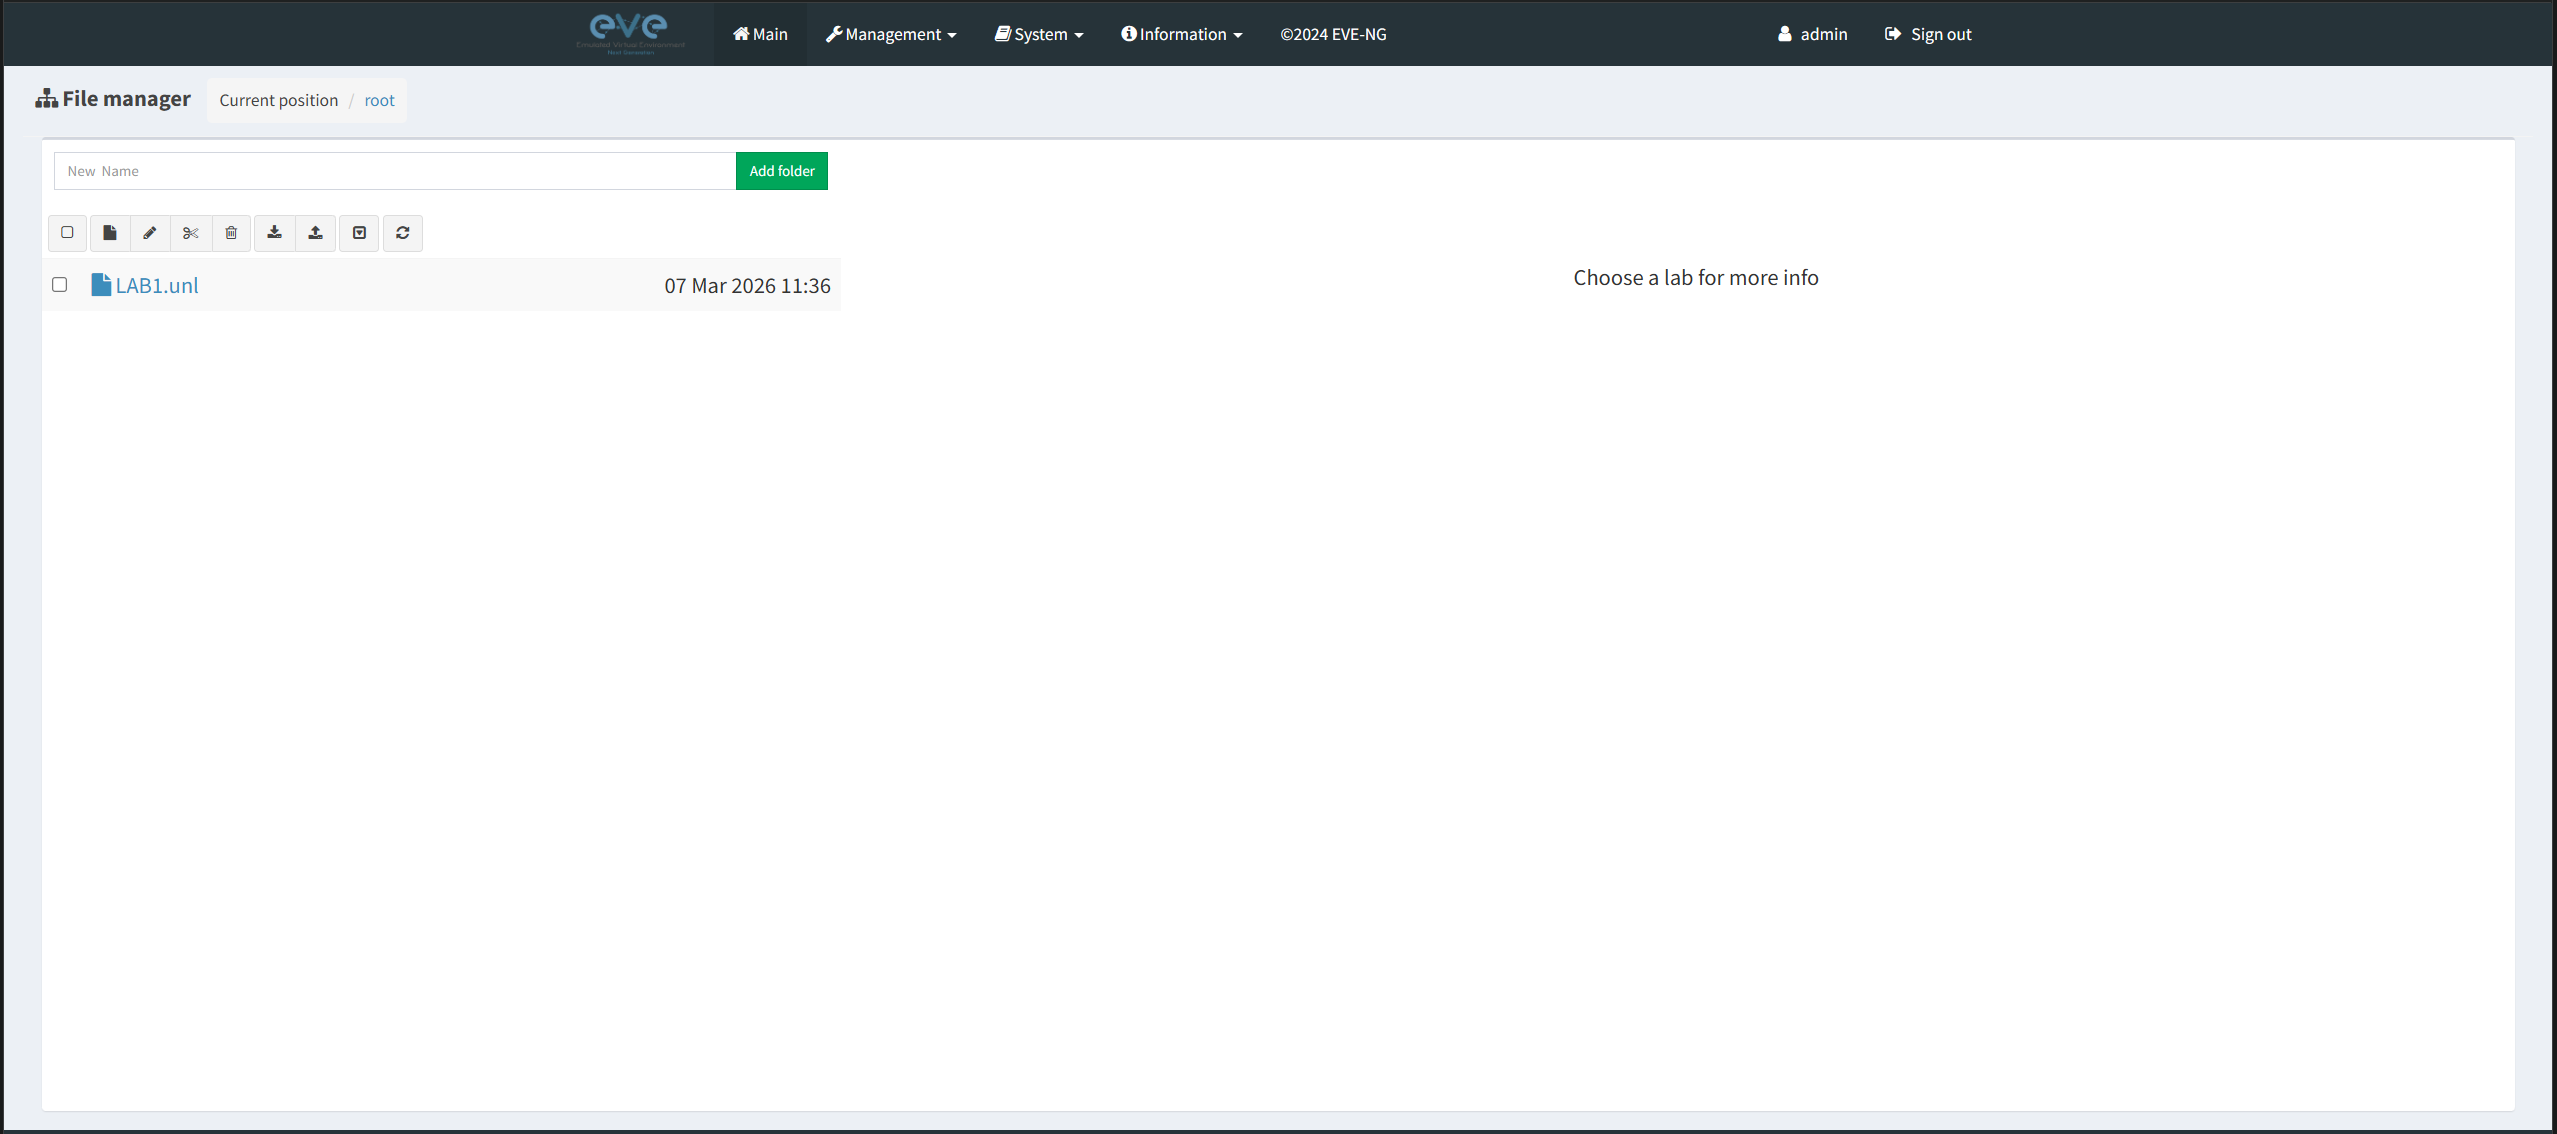
\includegraphics[width=0.9\textwidth]{eve-file-manager.png}
    \caption{EVE-NG File Manager showing the lab directory structure, import
             controls, and topology thumbnails.}
    \label{fig:eve-file-manager}
\end{figure}

The export format also simplifies distribution: a \texttt{.unl} file committed to
the project repository can be imported into any compatible EVE-NG instance,
reproducing the full topology without manual reconfiguration.


% ------------------------------------------------------------
\section{Infrastructure Problems}
% ------------------------------------------------------------

Several problems were encountered at the infrastructure level during the setup of
the EVE-NG environment. These are distinct from the lab-specific issues documented
within each lab section and relate to the underlying platform and tooling.

\subsection{EVE-NG on VMware}

The initial deployment target was a VMware-based server available through the
university. Despite EVE-NG being officially listed as compatible with VMware~\cite{vmware_esxi}
hypervisors, the environment produced recurrent instability: nodes failed to start
consistently, VNC sessions dropped without warning, and network connectivity between
virtual bridges was unreliable. No stable configuration was found after several
iterations. The root cause was not fully identified, but the combination of
VMware's nested virtualisation restrictions and the specific hardware and software
versions in the university environment appeared to be contributing factors.
The decision to migrate to Proxmox resolved all of these issues.

\subsection{Node Configuration Persistence}

A recurring challenge in EVE-NG lab design is ensuring that node configurations
survive restarts. By default, runtime network settings applied inside guest virtual
machines are lost when the lab is stopped or the EVE-NG host is rebooted. This
affected multiple nodes across the lab and required a dedicated solution for each
one. The specific mechanisms used are described in the relevant lab sections; the
general principle adopted throughout the project was to rely on the native
persistence mechanisms of each operating system --- such as \texttt{systemd-networkd}
unit files, NetworkManager connection profiles, and \texttt{udev} rules --- rather
than applying settings interactively at the console.

\subsection{LVM Volume Group Naming Conflict}

During a session involving disk operations on guest virtual machine images mounted
from the EVE-NG host, a naming conflict arose between the host's LVM volume group
and a guest disk's volume group, both named \texttt{ubuntu-vg}. An attempt to
resolve the conflict by renaming the host volume group caused the EVE-NG host to
fail on the next restart, dropping into an \texttt{initramfs} prompt because the
boot configuration still referenced the original group name.

Recovery was performed from the \texttt{initramfs} shell by renaming the volume
group back to its original name and reactivating it before resuming the normal boot
sequence. As a result of this incident, the rule established for the project is to
never rename a volume group belonging to the host operating system. When a naming
conflict arises with a guest disk, only the guest volume group is renamed, using a
descriptive identifier that includes the lab and node reference.

\subsection{Memory Capacity Constraint}

During concurrent development of the first two laboratories, peak memory
consumption on the EVE-NG virtual machine regularly exceeded the initial
32\,GB RAM allocation of the host server. Running pfSense, VyOS, Ubuntu Server,
Ubuntu Desktop, and Parrot OS simultaneously --- alongside other services
co-hosted on the same Proxmox infrastructure (monitoring stack, reverse proxy,
storage services) --- produced memory pressure that caused nodes to be killed
by the hypervisor's out-of-memory handler, interrupting development sessions.

An additional 32\,GB RAM module was acquired and installed, bringing the host
to 64\,GB total. This resolved the stability issues and allowed all lab nodes
to run concurrently without further intervention. The upgrade was not included
in the original project budget estimate; its approximate cost
(\textasciitilde 80\,\euro) is noted in Chapter~6 as a post-planning expenditure.


% ------------------------------------------------------------
\section{Lab Topologies}
% ------------------------------------------------------------

Four penetration testing lab topologies were designed for the course. Each topology
is implemented as an EVE-NG \texttt{.unl} file and can be imported into any
compatible EVE-NG instance. Table~\ref{tab:lab-overview} summarises the four labs,
their primary learning objective, and their current implementation status.

\begin{table}[h]
\centering
\small
\setlength{\tabcolsep}{5pt}
\begin{tabularx}{\textwidth}{@{}lXl@{}}
\toprule
\textbf{Lab} & \textbf{Primary Objective} & \textbf{Status} \\
\midrule
Lab~1: Reconnaissance \& Enumeration & Port scanning, web content discovery, SSH & Implemented \\
Lab~2: Web Application Vulnerabilities & OWASP Top~10 exploitation & Implemented \\
Lab~3: Network Analysis & Traffic capture, lateral movement, incident response & Implemented \\
Lab~4: Privilege Escalation & Local privilege escalation techniques & Pending \\
\bottomrule
\end{tabularx}
\caption{Overview of the four EVE-NG lab topologies designed for the course.}
\label{tab:lab-overview}
\end{table}

The remainder of this chapter describes each implemented lab in detail, covering
the network topology, design decisions, student workflow, and problems encountered
during development.


% ------------------------------------------------------------
% Lab descriptions --- one file per lab
% ------------------------------------------------------------
% Lab 1 --- compact version (full docs: docs/web/docs/labs/lab1/)
\section{Lab 1: Reconnaissance and Enumeration}

Lab~1 introduces the reconnaissance phase of a penetration test following the PTES
framework~\cite{ptes}. Students interact with a fictional target organisation,
\textit{PEBCAK Corp}, through a layered topology that includes a perimeter firewall
(pfSense~CE~\cite{pfsense}), an internal router (VyOS~\cite{vyos}), and a target
Ubuntu~Server~24.04~\cite{ubuntu}. Access is exclusively via DNS hostname
(\texttt{lab1}) resolved through pfSense's Unbound resolver~\cite{unbound_dns}, requiring students
to use proper service enumeration before any exploitation attempt. A teacher reference --- credentials, network table, and startup checklist --- is compiled
in Appendix~B; the complete topology, configuration files, and step-by-step guide are at
\path{docs/web/docs/labs/lab1/}.


\begin{figure}[H]
\centering
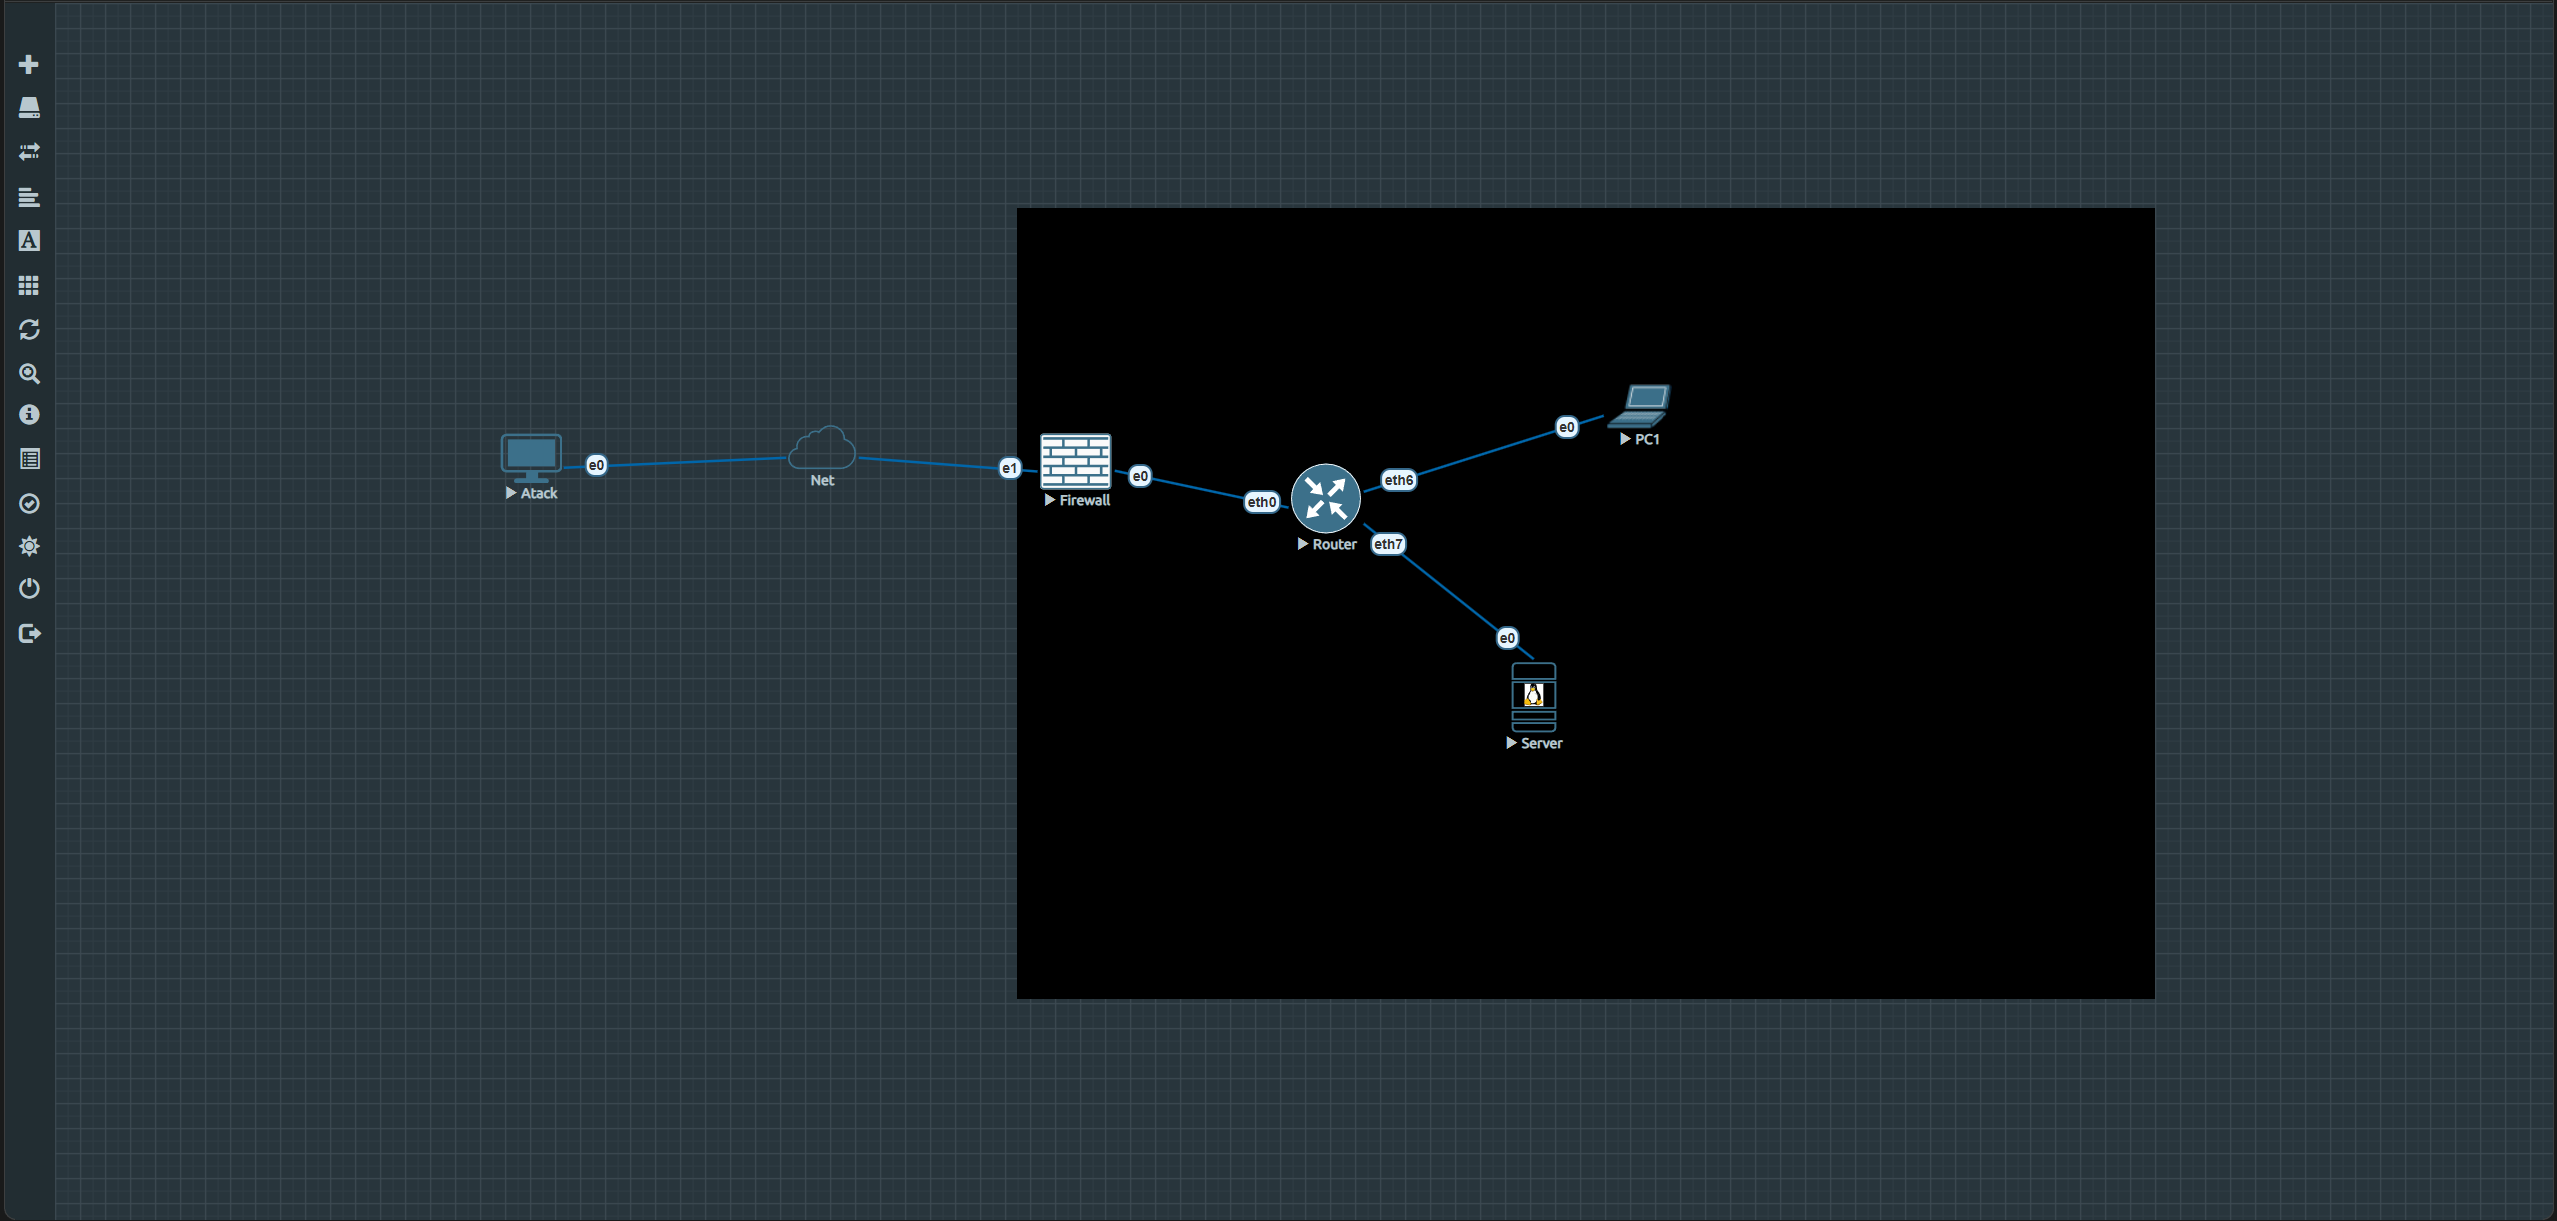
\includegraphics[width=0.95\textwidth]{lab1-topology.png}
\caption{Lab~1 network topology}
\label{fig:lab1-topology}
\end{figure}

\newpage
\subsubsection*{Network Addressing}

\begin{table}[H]
\centering
\resizebox{\textwidth}{!}{\begin{tabular}{@{}lllll@{}}
\toprule
\textbf{Node} & \textbf{Role} & \textbf{Interface} & \textbf{IP} & \textbf{Network} \\
\midrule
Parrot-OS   & Attacker        & eth0 & 192.168.0.x (DHCP) & 192.168.0.0/24 (Homelab)  \\
pfSense     & Firewall/NAT    & WAN  & 192.168.0.29       & 192.168.0.0/24            \\
pfSense     & Firewall/NAT    & LAN  & 172.16.0.1         & 172.16.0.0/30             \\
VyOS        & Router/L3       & eth0 & 172.16.0.2         & 172.16.0.0/30             \\
VyOS        & Router/L3       & eth6 & 192.168.10.5       & 192.168.10.0/24 (Users)   \\
VyOS        & Router/L3       & eth7 & 192.168.20.1       & 192.168.20.0/24 (Servers) \\
Server      & Target (web+SSH)& eth0 & 192.168.20.50      & 192.168.20.0/24           \\
PC1         & Workstation     & eth0 & 192.168.10.50      & 192.168.10.0/24           \\
\bottomrule
\end{tabular}}
\caption{Lab~1 IP addressing scheme}
\label{tab:lab1-ip}
\end{table}

\subsubsection*{Techniques and Framework Alignment}

\begin{table}[H]
\centering
\small
\begin{tabularx}{\textwidth}{lXl}
\toprule
\textbf{Technique} & \textbf{Description} & \textbf{Reference} \\
\midrule
DNS resolution        & Hostname-to-IP via Unbound resolver (RFC~1035~\cite{rfc1035}) & PTES Recon  \\
Port scanning         & TCP SYN scan with Nmap (RFC~793~\cite{rfc793})                & PTES Recon  \\
Service enumeration   & Banner grabbing, version detection                            & PTES Recon  \\
Web content discovery & Directory brute-force with Gobuster                           & OWASP WSTG  \\
Credential retrieval  & Exposed credentials in web content                            & OWASP A05:2021\\
SSH access            & Password-based login (RFC~4252~\cite{rfc4252})                & PTES Exploit\\
\bottomrule
\end{tabularx}
\caption{Lab~1 techniques and framework mapping}
\label{tab:lab1-techniques}
\end{table}

\subsection{Problems Encountered and Solutions}

\subsubsection{VNC Keyboard Input on QEMU Nodes}

EVE-NG provides VNC console access to QEMU nodes, but certain key combinations ---
most notably \texttt{Ctrl+C} and special characters such as \texttt{|}, \texttt{@},
and \texttt{\{} --- are not reliably forwarded by the browser-based VNC client or by
the \texttt{vncdo} command-line tool. The root cause was that vncdo sent key symbols
rather than raw key codes, and the VNC server's key mapping did not cover all
combinations used in a penetration testing context.

The solution was to inject keystrokes directly via the QEMU monitor socket,
using Python's raw socket interface to send \texttt{sendkey} commands. This bypasses
the VNC protocol entirely and ensures that arbitrary key sequences, including those
involving modifier keys, are delivered correctly to the guest.

\subsubsection{pfSense DNS Resolver WAN Interface}

After initial configuration, DNS queries from the attacker machine were not being
resolved by pfSense's Unbound resolver. The problem was that Unbound, by default,
only listens on the LAN interface, so queries arriving on the WAN-side interface
were silently discarded. The fix was to explicitly add the WAN interface to
Unbound's listening configuration under \textit{Services $\to$ DNS Resolver $\to$
Network Interfaces}.

\subsubsection{Unbound Startup Configuration Path}

On subsequent restarts, the Unbound configuration applied via the
GUI was not being preserved, causing DNS resolution to fail after every reboot.
Investigation revealed that pfSense's startup scripts write the Unbound configuration
to \path{/var/unbound/unbound.conf} at boot time, overwriting any manual edits.
The correct approach is to configure all resolver settings exclusively through the
GUI or through pfSense's \texttt{/etc/inc/} PHP hooks, never by editing the
generated configuration file directly.

\subsubsection{VyOS Source NAT Requirement}

Traffic routed through VyOS from the attacker to the target was being dropped
because the target's default gateway was pfSense, not VyOS. Return packets were
therefore routed back via pfSense rather than through VyOS, breaking the connection.
The fix was to configure Source NAT (masquerade) on VyOS for traffic entering
the internal segment, ensuring that return traffic would follow the same path back
through the VyOS router.

\subsubsection*{Results}

\begin{table}[H]
\centering
\resizebox{\textwidth}{!}{\begin{tabular}{@{}lll@{}}
\toprule
\textbf{Flag} & \textbf{Location} & \textbf{Technique} \\
\midrule
\texttt{FLAG\{p3bc4k\_s3rv3r\_0wn3d\}} & \texttt{\textasciitilde/flag.txt} on Server via SSH & Credentials from hidden web page \\
\texttt{FLAG\{d3f4ult\_cr3ds\_k1ll\_s3cur1ty\}} & \texttt{/root/flag.txt} on pfSense via SSH pivot & Default credentials \\
\texttt{FLAG\{sk1n3t\_b3c4m3\_s3nt13nt\}} & \texttt{\textasciitilde/flag.txt} on PC1 via lateral move & Credentials found in pfSense flag \\
\bottomrule
\end{tabular}}
\caption{Lab~1 flags and acquisition techniques}
\label{tab:lab1-flags}
\end{table}

% Lab 2 --- compact version (full docs: docs/web/docs/labs/lab2/)
\section{Lab 2: Web Application Vulnerabilities --- SYNAPSE Intelligence Portal}

Lab~2 presents students with a custom two-tier web application,
\textit{SYNAPSE Intelligence Portal}, deployed on a segmented DMZ architecture.
The scenario is aligned with the OWASP Top~10~\cite{owasp2021} and chains
multiple vulnerabilities across two servers: Server-A hosts the portal front-end
with authentication and reporting features; Server-B hosts the DataVault internal
file management service accessible only after pivoting from Server-A. Students must
complete a progressive exploitation chain --- stored XSS, cookie theft, SQL injection,
and YAML deserialization --- to collect all three flags. A teacher reference --- credentials, startup procedure, and flag guide --- is compiled in Appendix~C;
complete source code, topology, and deployment instructions are at \path{docs/web/docs/labs/lab2/}.


\begin{figure}[H]
\centering
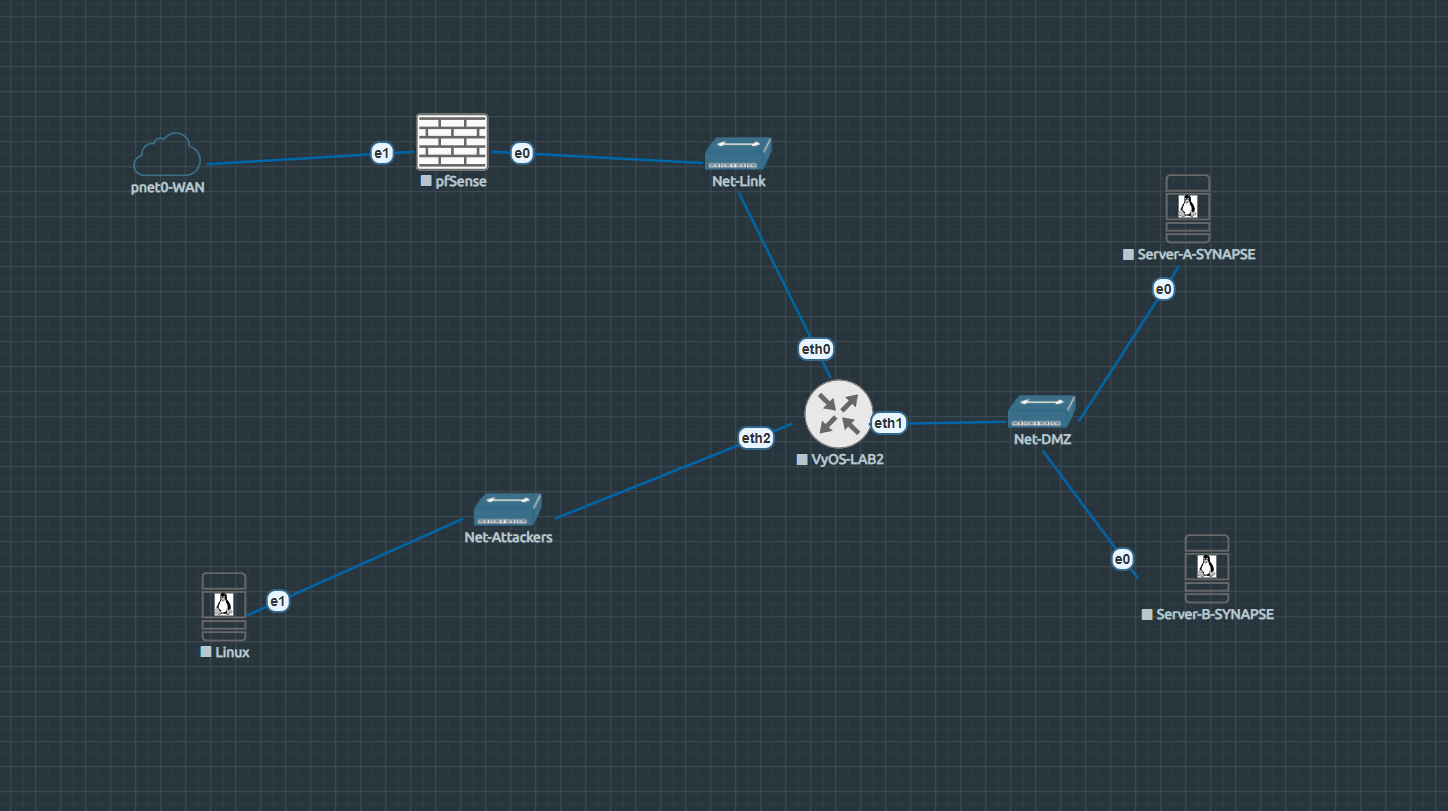
\includegraphics[width=0.95\textwidth]{lab2-topology.png}
\caption{Lab~2 network topology}
\label{fig:lab2-topology}
\end{figure}

\subsubsection*{Network Addressing}

\begin{table}[H]
\centering
\resizebox{\textwidth}{!}{\begin{tabular}{@{}lllll@{}}
\toprule
\textbf{Node} & \textbf{Role} & \textbf{Interface} & \textbf{IP} & \textbf{Network} \\
\midrule
Parrot-OS    & Attacker          & eth0  & 10.0.40.10       & 10.0.40.0/24 (Net-Attackers) \\
pfSense-LAB2 & Firewall/NAT      & WAN   & 192.168.0.x (DHCP) & 192.168.0.0/24 (Homelab)   \\
pfSense-LAB2 & Firewall/NAT      & LAN   & 172.16.1.1       & 172.16.1.0/30              \\
VyOS-LAB2    & DMZ Router        & eth0  & 172.16.1.2       & 172.16.1.0/30              \\
VyOS-LAB2    & DMZ Router        & eth1  & 192.168.30.1     & 192.168.30.0/24 (Net-DMZ)  \\
VyOS-LAB2    & DMZ Router        & eth2  & 10.0.40.1        & 10.0.40.0/24 (Net-Attackers)\\
Server-A     & SYNAPSE Portal    & eth0  & 192.168.30.10    & 192.168.30.0/24            \\
Server-B     & DataVault         & eth0  & 192.168.30.20    & 192.168.30.0/24            \\
\bottomrule
\end{tabular}}
\caption{Lab~2 IP addressing scheme}
\label{tab:lab2-ip}
\end{table}

\subsubsection*{OWASP Coverage and Vulnerability Chain}

\begin{table}[H]
\centering
\small
\begin{tabularx}{\textwidth}{llXl}
\toprule
\textbf{Step} & \textbf{OWASP} & \textbf{Vulnerability} & \textbf{Flag} \\
\midrule
1 & A03:2021 & Stored XSS in report field $\rightarrow$ session cookie theft & -- \\
2 & A07:2021 & Cookie injection $\rightarrow$ admin panel access & -- \\
3 & A03:2021 & SQL injection in search $\rightarrow$ credential dump & FLAG\{synapse\_sqli\_creds\_dumped\} \\
4 & A01:2021 & Lateral movement to Server-B via stolen creds & FLAG\{synapse\_pivot\_server\_b\} \\
5 & A08:2021 & YAML deserialization in DataVault upload $\rightarrow$ RCE & FLAG\{synapse\_rce\_achieved\} \\
\bottomrule
\end{tabularx}
\caption{Lab~2 OWASP Top~10 vulnerability chain}
\label{tab:lab2-vulns}
\end{table}

\subsubsection*{Results}

All three flags were successfully captured, confirming the complete exploitation
chain from stored XSS to remote code execution.

\begin{table}[H]
\centering
\resizebox{\textwidth}{!}{\begin{tabular}{@{}lll@{}}
\toprule
\textbf{Flag} & \textbf{Location} & \textbf{Technique} \\
\midrule
\texttt{FLAG\{synapse\_sqli\_creds\_dumped\}} & \texttt{/search?q=} UNION dump on Server-A & UNION SQL Injection \\
\texttt{FLAG\{synapse\_pivot\_server\_b\}}    & \texttt{/home/monitor/flag.txt} on Server-B & SSH pivot with SQLi-extracted credentials \\
\texttt{FLAG\{synapse\_rce\_achieved\}}       & \texttt{/preview} reverse shell on Server-B  & YAML deserialization RCE \\
\bottomrule
\end{tabular}}
\caption{Lab~2 flags and acquisition techniques}
\label{tab:lab2-flags}
\end{table}

\newpage

\subsection{Problems Encountered and Solutions}

\subsubsection{pfSense Block Private Networks and Reply-To}

Two pfSense default behaviours blocked traffic in the lab topology. First, the
\textit{Block private networks} option on the WAN interface was enabled by default,
causing pfSense to silently discard packets arriving from the simulated
attacker network (RFC~1918 space~\cite{rfc1918}). Second, the \textit{Reply-to}
feature added return routes in \texttt{pf} rules that conflicted with VyOS's
routing table, causing asymmetric routing. Both were disabled: the private network
block via the WAN interface settings, and reply-to via a per-rule option in the
firewall rule editor.

\subsubsection{VNC Keyboard Input on pfSense}

The same VNC key injection issue documented in Lab~1 reappeared on pfSense
console sessions, particularly when entering characters required by the pfSense
shell (\texttt{|}, \texttt{\&}, \texttt{\$}). The QEMU monitor raw socket approach
was applied identically.

\subsubsection{Server-A Volume Group Conflict}

When mounting the Server-A QCOW2 image from the EVE-NG host to pre-stage
application files, the host's own LVM volume group (\texttt{ubuntu-vg}) conflicted
with the guest disk's identically named group. Activating both simultaneously
caused the host's logical volumes to be shadowed. The solution was to rename the
guest volume group to \texttt{synapse-vg} using \texttt{vgrename} before activating
it on the host, then rename it back after dismounting.

\subsubsection{Server-B Installer Keyboard Layout}

During the Server-B installation, the Ubuntu installer defaulted to a Spanish
keyboard layout due to the locale of the EVE-NG host, causing mismatched characters
when entering the initial credentials. This was corrected by explicitly selecting the
\texttt{en\_US} keyboard layout at the installer prompt and verified with a
\texttt{/dev/urandom}-seeded password test before proceeding.

\subsubsection{Static Route Gateway Reference}

VyOS rejected a static route configuration that referenced a gateway IP not directly
reachable on any configured interface. The intended next-hop was on a subnet not yet
assigned to any VyOS interface at the time the route was applied. This was resolved
by defining the interface address before the static route, and by using
\texttt{commit} and \texttt{save} in the correct order within the VyOS configuration
session.


% Lab 3 --- compact version (full docs: docs/web/docs/labs/lab3/)
\section{Lab 3: Incident Response and Log Forensics --- HELIX Systems}

Lab~3 inverts the student's role: instead of attacking, they act as a security
analyst responding to an active incident at \textit{HELIX Systems}. The lab
environment comes pre-staged with evidence of a simulated intrusion --- brute-force
SSH attempts, a successful login, privilege escalation via \texttt{sudo}
misconfiguration, backdoor account creation, and lateral movement to a database
server. Students must reconstruct the attack timeline from system logs
(\texttt{auth.log}, \texttt{bash\_history}) and identify the attacker's actions
and impact, following a methodology aligned with NIST SP~800-61~\cite{nist_sp80061}.
A quick teacher reference --- account table, attack timeline, and startup checklist --- is compiled in Appendix~D;
the full evidence walkthrough, forensic guide, and deployment instructions are at \path{docs/web/docs/labs/lab3/}.


\begin{figure}[H]
\centering
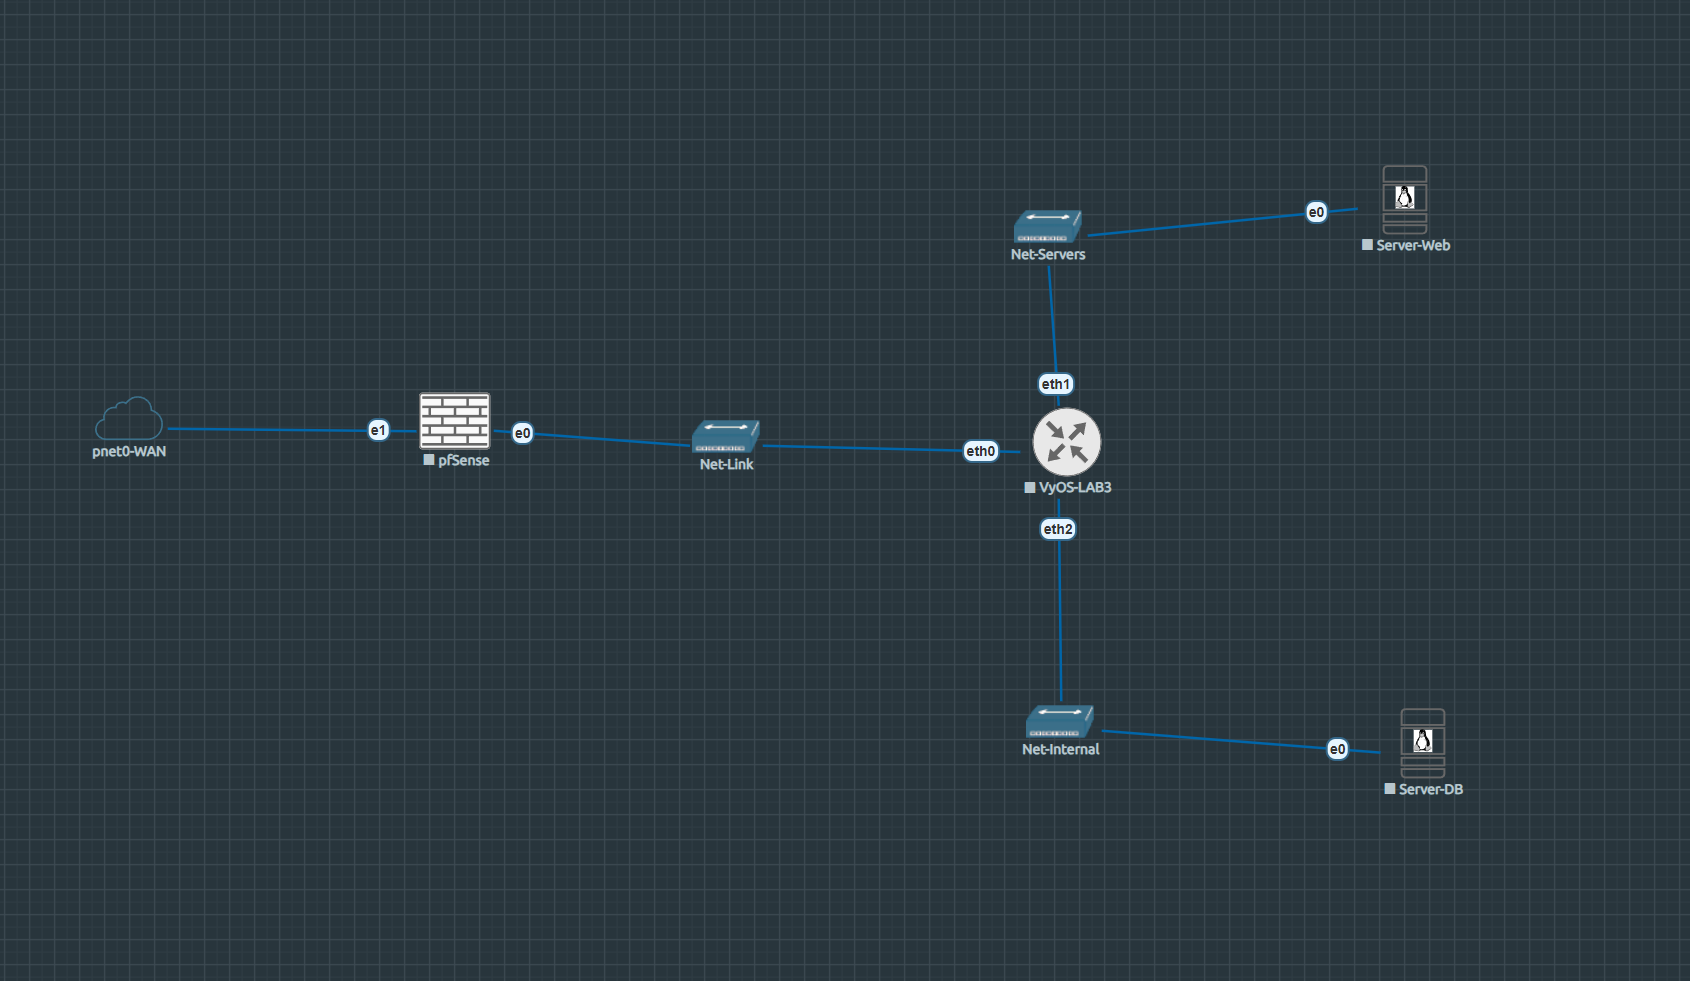
\includegraphics[width=0.95\textwidth]{lab3-topology.png}
\caption{Lab~3 network topology}
\label{fig:lab3-topology}
\end{figure}

\subsubsection*{Network Addressing}

\begin{table}[H]
\centering
\resizebox{\textwidth}{!}{\begin{tabular}{@{}lllll@{}}
\toprule
\textbf{Node} & \textbf{Role} & \textbf{Interface} & \textbf{IP} & \textbf{Network} \\
\midrule
Parrot-OS    & Analyst station   & eth0  & 192.168.0.x (DHCP) & 192.168.0.0/24 (Homelab)       \\
pfSense-LAB3 & Firewall/DNAT     & WAN   & 192.168.0.x (DHCP) & 192.168.0.0/24                 \\
pfSense-LAB3 & Firewall          & LAN   & 172.16.2.1         & 172.16.2.0/30                  \\
VyOS-LAB3    & Internal router   & eth0  & 172.16.2.2         & 172.16.2.0/30                  \\
VyOS-LAB3    & Internal router   & eth1  & 192.168.50.1       & 192.168.50.0/24 (Net-Servers)  \\
VyOS-LAB3    & Internal router   & eth2  & 192.168.60.1       & 192.168.60.0/24 (Net-Internal) \\
Server-Web   & Compromised web   & eth0  & 192.168.50.10      & 192.168.50.0/24                \\
Server-DB    & Internal DB       & eth0  & 192.168.60.10      & 192.168.60.0/24                \\
\bottomrule
\end{tabular}}
\caption{Lab~3 IP addressing scheme}
\label{tab:lab3-ip}
\end{table}

\subsubsection*{MITRE ATT\&CK Coverage}

\begin{table}[H]
\centering
\small
\begin{tabularx}{\textwidth}{llX}
\toprule
\textbf{MITRE ID} & \textbf{Technique} & \textbf{Evidence in lab} \\
\midrule
T1110.001 & Brute Force: Password Guessing & \texttt{auth.log} failed attempts \\
T1078     & Valid Accounts                 & \texttt{devops} account compromise \\
T1548.003 & Abuse Elevation Control Mechanism: Sudo and Sudo Caching          & NOPASSWD rule for \texttt{find} in \texttt{sudoers.d/devops} \\
T1136.001 & Create Account: Local          & Backdoor \texttt{maint} account \\
T1021.004 & Remote Services: SSH           & Lateral movement to Server-DB \\
T1005     & Data from Local System         & \texttt{/opt/helix/data/} exfil marker \\
\bottomrule
\end{tabularx}
\caption{Lab~3 MITRE ATT\&CK technique coverage}
\label{tab:lab3-mitre}
\end{table}

\newpage
\subsubsection*{Forensic Findings}

\begin{table}[H]
\centering
\small
\resizebox{\textwidth}{!}{\begin{tabular}{@{}lll@{}}
\toprule
\textbf{Finding} & \textbf{Artefact / Location} & \textbf{Host} \\
\midrule
Brute-force source (\texttt{185.220.101.47}) & \texttt{/var/log/auth.log} --- 25 failed SSH for \texttt{devops} & Server-Web \\
Initial compromise (03:17)   & \texttt{auth.log} successful login as \texttt{devops}                                        & Server-Web \\
Privilege escalation (03:18) & \texttt{sudo /usr/bin/find} NOPASSWD; \texttt{auth.log} + \texttt{/etc/sudoers.d/devops}    & Server-Web \\
Backdoor persistence (03:19) & \texttt{useradd maint}; \texttt{/etc/passwd} + \texttt{/etc/sudoers.d/maint}                 & Server-Web \\
Attacker commands            & \texttt{/home/devops/.bash\_history}                                                         & Server-Web \\
Lateral movement (03:21)     & \texttt{auth.log} \texttt{devops} SSH from \texttt{192.168.50.10}                            & Server-DB  \\
Data exfiltration (03:22)    & \texttt{/opt/helix/data/.exfil\_marker} + \texttt{clients.db}                               & Server-DB  \\
\bottomrule
\end{tabular}}
\caption{Lab~3 forensic findings and evidence locations (all timestamps UTC as recorded in \texttt{/var/log/auth.log})}
\label{tab:lab3-findings}
\end{table}

\subsection{Problems Encountered and Solutions}

\subsubsection{LVM Volume Group Naming Conflict}

When pre-staging Server-Web's evidence files from the EVE-NG host, the same
volume group conflict from Lab~2
recurred: both the host and the guest disk used \texttt{ubuntu-vg}. The resolution
procedure was identical --- renaming the guest VG to \texttt{helix-web-vg} before
activation --- and the naming rule was formally added to the project's infrastructure
runbook to prevent recurrence in future labs.

\subsubsection{Read-only NBD Device}

On one occasion, the QCOW2 image mounted via \texttt{qemu-nbd} was presented as
read-only despite the absence of the \texttt{--read-only} flag. Investigation revealed that a
previous mount session had not been cleanly disconnected (\texttt{qemu-nbd~-{}-disconnect}), leaving the kernel's NBD client in an inconsistent state.
The fix was to explicitly disconnect any stale NBD device before re-mounting, and
to add a pre-mount check to the project's image manipulation scripts.

\subsubsection{Analyst Group Membership for Log Access}

The student account (\texttt{analyst}) was created with restricted permissions so
that it could not read system logs directly without elevated group membership. However, \texttt{/var/log/auth.log}
requires membership of the \texttt{adm} group on Ubuntu. The pre-staging script was
updated to add \texttt{analyst} to \texttt{adm} at image preparation time, preserving
the educational constraint (no \texttt{sudo} to \texttt{root}) while allowing access
to the evidence files that are the focus of the lab.

\subsubsection{pfSense Console Access via QEMU Monitor}

The pfSense serial console was inaccessible through the standard EVE-NG Telnet
interface due to a configuration mismatch between the QEMU serial port definition
and pfSense's expected console device (\texttt{ttyu0} vs \texttt{ttyS0}). Console
access was recovered by connecting directly to the QEMU monitor socket and issuing
a \texttt{sendkey} sequence to navigate the pfSense boot menu, where the console
port assignment could be corrected persistently.



% ============================================================================
% BIBLIOGRAPHY
% ============================================================================


\clearpage
\phantomsection
\addcontentsline{toc}{chapter}{Bibliography}
\printbibliography


% Include time log appendix if it exists (avoids build failures if missing)

\appendix
\clearpage



\end{document}










